\documentclass[preprint,
3p]{elsarticle} %review=doublespace preprint=single 5p=2 column
%%% Begin My package additions %%%%%%%%%%%%%%%%%%%

\usepackage[hyphens]{url}

  \journal{Journal of Computational Science} % Sets Journal name

\usepackage{graphicx}
%%%%%%%%%%%%%%%% end my additions to header

\usepackage[T1]{fontenc}
\usepackage{lmodern}
\usepackage{amssymb,amsmath}
% TODO: Currently lineno needs to be loaded after amsmath because of conflict
% https://github.com/latex-lineno/lineno/issues/5
\usepackage{lineno} % add
\usepackage{ifxetex,ifluatex}
\usepackage{fixltx2e} % provides \textsubscript
% use upquote if available, for straight quotes in verbatim environments
\IfFileExists{upquote.sty}{\usepackage{upquote}}{}
\ifnum 0\ifxetex 1\fi\ifluatex 1\fi=0 % if pdftex
  \usepackage[utf8]{inputenc}
\else % if luatex or xelatex
  \usepackage{fontspec}
  \ifxetex
    \usepackage{xltxtra,xunicode}
  \fi
  \defaultfontfeatures{Mapping=tex-text,Scale=MatchLowercase}
  \newcommand{\euro}{€}
\fi
% use microtype if available
\IfFileExists{microtype.sty}{\usepackage{microtype}}{}
\usepackage[]{natbib}
\bibliographystyle{elsarticle-num-names}

\ifxetex
  \usepackage[setpagesize=false, % page size defined by xetex
              unicode=false, % unicode breaks when used with xetex
              xetex]{hyperref}
\else
  \usepackage[unicode=true]{hyperref}
\fi
\hypersetup{breaklinks=true,
            bookmarks=true,
            pdfauthor={},
            pdftitle={Exploring Network-Level Indicators for Project Analysis - A Comparison of Real and Synthetic Projects},
            colorlinks=false,
            urlcolor=blue,
            linkcolor=magenta,
            pdfborder={0 0 0}}

\setcounter{secnumdepth}{5}
% Pandoc toggle for numbering sections (defaults to be off)


% tightlist command for lists without linebreak
\providecommand{\tightlist}{%
  \setlength{\itemsep}{0pt}\setlength{\parskip}{0pt}}




\usepackage{subfig}
\usepackage{float}
\usepackage[utf8]{inputenc}
\usepackage{appendix}
\renewcommand{\appendixname}{Supplementary Material}
\renewcommand{\thesection}{\arabic{section}}
\DeclareUnicodeCharacter{3B1}{\ensuremath{\alpha}}
\usepackage{multibib}
\newcites{supp}{Supplementary References}
\let\<\textless
\let\>\textgreater
\usepackage{booktabs}
\usepackage{longtable}
\usepackage{array}
\usepackage{multirow}
\usepackage{wrapfig}
\usepackage{float}
\usepackage{colortbl}
\usepackage{pdflscape}
\usepackage{tabu}
\usepackage{threeparttable}
\usepackage{threeparttablex}
\usepackage[normalem]{ulem}
\usepackage{makecell}
\usepackage{xcolor}



\begin{document}


\begin{frontmatter}

  \title{Exploring Network-Level Indicators for Project Analysis - A
Comparison of Real and Synthetic Projects}
    \author[University of Pannonia, Institute of Advanced Studies
Kőszeg]{Zsolt T. Kosztyán%
  \corref{cor1}%
  }
   \ead{kosztyan.zsolt@gtk.uni-pannon.hu} 
      \cortext[cor1]{Corresponding author}
  
  \begin{abstract}
  This study introduces a novel perspective on project network analysis
  by incorporating network theory and graph analysis to identify
  network-level indicators for activity-on-node project networks. A key
  contribution lies in the comparison between real and synthetic
  projects on the basis of project and network-level indicators,
  revealing distinct variations. The findings underscore that real
  projects demonstrate lower flexibility and efficiency than synthetic
  counterparts, impacting project scheduling and resource allocation.
  Moreover, the study suggests employing supervised and unsupervised
  learning classification methods to categorize projects on the basis of
  indicator values, enhancing project selection and prioritization
  processes. By bridging the gap between network-level indicators and
  project aspects, this research enriches the literature by offering
  fresh insights and resources for project managers to optimize project
  network structure and performance.
  \end{abstract}
    \begin{keyword}
    network indicators \sep project database \sep synthetic
projects \sep 
    real project structures
  \end{keyword}
  
 \end{frontmatter}

\sloppy

\section{Introduction}\label{sec:intro}

The significance of projects is crucial and includes several aspects,
such as corporate operations, research, and national economies
\citep{DENIZER2013projGDP}. Within the project management,the project
planning problem is a critical challenge in management science and
operations research, focusing on efficient scheduling and resource
allocation of project activities \citep{hartmann2022updated}. This
complex task involves organizing interconnected activities, managing
resources, and optimizing project timelines to achieve the desired
outcomes. The significance of project planning extends across various
domains, including corporate operations, research initiatives, and
national economies. Researchers in Management Science and Operations
Research have thoroughly examined project scheduling and resource
allocation for more than sixty years \citep{Franco2019review}. Project
databases were suggested as a means to evaluate algorithms, encompassing
both simulated \citep{boctor1993heuristics} and real scenarios
\citep{batselier2015construction}, as well as individual
\citep{sprecher1996psplib} or multiple projects
\citep{browning2010random}, and single-mode
\citep{patterson1984comparison} or multimode projects
\citep{Vanpeteghem2014}. Nevertheless, the numerous project databases
exhibit significant heterogeneity in terms of both the file structure
and the characteristics of the represented projects.
\citet{kosztyan2023matrix} proposed a unified matrix-based project
planning (UMP) model, which offers several advantages over existing
network-based project planning methods and heterogeneous network-based
sources of project plans. UMP provides a unified approach that can
seamlessly represent both individual projects and multiprojects
portfolios. It is scalable in terms of complexity and is capable of
handling both single-mode and multimode project completions. Moreover,
UMP's power lies in its ability to collect and integrate most existing
projects databases, allowing for comprehensive analysis and comparison
across diverse project structures and datasets. This unified framework
enables researchers and project managers to conduct more robust and
standardized analyses, facilitating better understanding and management
of complex project networks. \citet{kosztyan2022mfpp} proposed a MATLAB
model, and \citet{mfpppkg} proposed an R package that can plan different
kinds of project scheduling problems. \citet{mfpppkg} stores
\citep{boctor1993heuristics}'s synthetic and
\citet{batselier2015construction}'s real-life projects. The logic
structure of the project is stored in a logic domain, which is an
adjacency matrix of the activity-on-node network of the project plan.
Further domains (i.e., submatrices) store the task duration and resource
demands by completion mode and resource type.

Owing to the UMP, different types of project databases can be compared
to each other. In addition, project networks can be analyzed by
network-level indicators. In this paper, we present the following
research questions.

\begin{description}
\item[$\mathbf{RQ}_1$\label{RQ1}] What are the new insights from the proposed network-level indicators for project planning and scheduling?
\item[$\mathbf{RQ}_2$\label{RQ2}] What is the relationship between the proposed network level and the existing project indicators?
\item[$\mathbf{RQ}_3$\label{RQ3}] What is the difference between real and synthetic project plans in the case of the project and network-level indicators?
\end{description}

The investigation of \nameref{RQ1} can facilitate the identification of
the prospective advantages and difficulties associated with the
utilization of network-level indicators for project planning and
scheduling. Network-level indicators refer to metrics that quantify the
qualities and attributes of the project network; these metrics include
density, diameter, modularity, centrality, resilience, efficiency, and
transitivity. Moreover, these metrics offer novel perspectives on the
composition and intricacy of the project network, as well as their
impact on project performance, risk, and quality. The examination of
\nameref{RQ2} can provide insights into the relationships in the
network-level indicators and the current project metrics. The existing
project indicators encompass many measurements that reflect key features
of project management, including duration, resource allocation, and
network complexity, order strength, activity distribution, and
topological float. These indicators can offer insights into the scope,
timing, cost, and logic of the project. An examination of the
correlation between network-level indicators and current project
indicators, the impact of network properties on project elements can be
understood along with the reciprocal influence. Additionally, methods
for integrating and for These factors can be aligned to enhance project
management. The use of \nameref{RQ3} allows direct comparison and
analysis of the project and network-level indicators between real and
synthetic project plans. Real project plans are derived from factual
data obtained from companies in various industries, whereas synthetic
project plans are produced by random network generators. The research
goal is to assess the accuracy and usefulness of the simulation model by
comparing the actual project plans with synthetic plans. Additionally,
we seek to uncover the commonalities and disparities between the real
and synthetic project networks.

The research questions were addressed as follows. The background of the
study, and the contributions of our study to the literature are as
follows: Section \ref{sec:background}. Methods and application materials
are as follows: introduced in Section \ref{sec:methods}. In Section
\ref{sec:results}, We report the results of the study. In Section
\ref{sec:discussion}, we discuss the results of the study. Section
\ref{sec:conclusion} provides the summary and conclusions, and finally,
Section \ref{sec:limitations} shows the limitations and potential
further directions.

\section{Background of the study}\label{sec:background}

A multitude of indicators are presented in the literature, as there are
continuous endeavors to create novel indicators. Vanhoucke provides a
comprehensive summary in \citet{vanhoucke2016overview}, and
\citet{browning2010resource} offer a comprehensive analysis of different
projects. \citet{van2020resource} and \citet{VANEYNDE2022853} have
expanded their research to incorporate indicators for both projects
generation and classification.

The existing indicators can be separated into three large groups: (1)
\emph{time-related}, (2) \emph{resource-related} and (3)
\emph{structural} (i.e.,. \emph{logic}) indicators (see the summary in
\citet{van2023summary}). The \emph{time-related indicators} measure the
duration, schedule, and flexibility of the project activities and the
project as a whole. These measures include variables such as average
activity duration, critical path length, number and percentage of
activities with positive slack, average slack and the slack ratio, and
variance in activity duration. They are important because they help to
monitor and control project progress, performance, and quality. (2) The
\emph{resource-related indicators} measure the allocation, utilization,
and diversity of project resources, such as human, material, or
financial resources. These variables include the number of renewable
resources, alpha distribution of resource strength, the normalized
average resource loading factor, and the resource leveling index. Such
measures are important because they help optimize project cost,
efficiency, and reliability. Finally, (3) \emph{structural (logical)
indicators} measure the complexity, order, and density of the project
network, which represents the activities and their dependencies in a
project. These structural indicators include variables such as the
network complexity coefficient, the order strength coefficient, the
activity distribution index, the serial/parallel index, the length of
the long arcs index, the short arcs index, the topological float index,
the total and average activity density, the number of articulation
points, and the number of components. These variables are important
because they help to understand the structure and logic of the project
network while improving project planning and scheduling.

Since structural indicators already incorporate the basic properties of
the project network, several network-level indicators are not
interpreted in the project network and are not used to describe the
logic structure of the project network.

A project network is also a network that is a set of nodes and a set of
edges that connect some pairs of nodes. In the case of an
Activity-on-Node (AoN) project network, the nodes represent tasks
(activities), and the edges represent dependencies. A dependency is a
logical relationship that specifies the order or sequence of the tasks.
An AoN project network is a directed network in which the edges have a
direction that indicates the precedence of the tasks. Such a network is
usually a directed acyclic graph (DAG), where there are no cycles or
loops in the network; however, our analysis does not require this
property.

Project indicators are crucial for delineating project frameworks, for
assessing structural intricacy, for estimating length, for identifying
idle time, and for determining resource requirements. This information
has the potential to significantly impact the performance of the
scheduling or resource allocation process \citep{van2023summary}.
Nevertheless, while these indicators are focused on time and resource
demands, and there are several indicators that focus on the project
structure of the project, to our knowledge, most network-level
indicators, such as centralization, modularity, and transitivity are not
considered. However, these indicators may provide new insights for the
project managers.

The main difference between the proposed network-level and structural
indicators is that the network-level indicators are on the basis of
network theory and graph analysis, while the structural indicators are
on the basis of project management theory and logic analysis. This means
that network-level indicators offer a more holistic and dynamic
perspective on the project network, whereas the structural indicators
offer a greater Detailed and static perspective on the project network.
Another The difference between the network-level and structural
indicators is that the network-level indicators capture the emergent and
nonlinear properties of the project network; these properties include
modularity, centrality, resilience, efficiency, and transitivity. The
structural indicators capture the deterministic and linear properties of
the project network, such as complexity, order, and density. This means
that the network-level indicators can reveal the hidden and unexpected
patterns and behaviors of the project network, whereas the structural
indicators can reveal the explicit and predictable rules and constraints
of the project network. For the structural indicators, it is assumed
that the project network is homogeneous, independent, and static; this
assumption may not reflect the reality of a complex and dynamic project
environment. Network-level indicators can address these limitations by
incorporating heterogeneity, interactivity, and adaptability of the
project network, which can lead to more realistic and robust project
network analysis.

To compare different kinds of project databases, we used the UMP model.
However, because of the focus on the project indicators, we consider
only logic (LD), time (TD) and (renewable) resource domains (RD), which
store the AoN project network, the time and the resource demands.

This study makes three contributions to the literature.

\begin{description}
\item[$\mathbf{C}_1$\label{C1}] We interpret network-level indicators to explain the logical structure of an activity-on-node network, and we demonstrate how these indications can be understood within the framework of a project.
\item[$\mathbf{C}_2$\label{C2}] We show the effects of the time-related, the resource-related, and the structural project metrics on the suggested network-level indicators.
\item[$\mathbf{C}_3$\label{C3}] We show that synthetic and real projects exhibit distinct variations in their project and network indicator values. These variables can therefore be employed to categorize projects with supervised and unsupervised learning classification techniques.
\end{description}

According to the contribution of \nameref{C1}, we propose a new
perspective on project network analysis that is on the basis of network
theory and graph analysis. Network-level indicators are measures that
capture the properties and characteristics of the project network, such
as density, diameter, modularity, centrality, resilience, efficiency,
and transitivity. These indicators can provide novel insights into how
connected, diverse, modular, centralized, resilient, efficient, and
cohesive the project network is, and how these factors affect project
performance, risk, and quality. Interpreting network-level indicators in
context of an activity-on-node network, we show how these indicators can
be applied and understood within the framework of a project.
Contribution \nameref{C2} regards the relationship between the
network-level indicators and the existing project indicators. Existing
project indicators are measures that capture the aspects of the project
time, resources, and logic. These indicators can provide information
about the project scope, schedule, and logic. By showing the effects
between the network-level indicators and the existing project
indicators, we reveal how the network properties influence and are
influenced by the project aspects and how they can be integrated and
aligned for better project management. Finally, according to
contribution \nameref{C3}, we compare and contrast the real and
synthetic project plans in terms of the project and network-level
indicators. Real project plans are on the basis of actual data, e.g.,
from a construction or a service-oriented company, while synthetic
project plans are generated by a random network generator. By
demonstrating that synthetic and real projects exhibit distinct
variations in their project and network indicators values, we evaluate
the validity and the applicability of the simulation model. Moreover, we
identify the similarities and differences between the real and synthetic
project networks. We also demonstrate how these variables can be used to
categorize projects with supervised and unsupervised learning
classification techniques, which can improve the project selection and
prioritization processes. This classification step highlights what are
the most different indicators between a real-life and synthetic
projects.

To achieve maximal reproducibility, this study used the R programming
language. The \textbf{rticles} \citep{rticlespkg} package was utilized
to generate the LaTeX code and the corresponding PDF document. All the
data and tables are derived from computations. The entire code is
provided alongside the publication to enable anyone to replicate the
findings. The following R packages are used in the paper: To read the
descriptive files of the indicators we used the \textbf{readxl} package
\citep{readxlpkg}. For the data preparation and manipulation, we used
the \textbf{xfun} \citep{xfunpkg}, \textbf{stringr} \citep{stringrpkg}
packages. For descriptive statistics, we used the \textbf{DescTools}
package \citep{DescToolspkg} and for analysis of variance (ANOVA), we
applied the \textbf{car} package \citep{carpkg}. For the cluster
analysis and unsupervised learning, we used the package \textbf{nda}
\citep{kosztyan2023network} and to calculate the multidimensional
scaling, we used the \textbf{MASS} package \citep{MASSpkg}. To measure
the average of the silhouette meusure, we used \textbf{cluster} package
\citep{clusterpkg}. In the case of supervised learning, we used
\textbf{Boruta} \citep{Borutapkg} to calculate relevant indicators, and
we used the \textbf{randomForest} package \citep{randomForestpkg} to
calculate variable importance. To calculate accuracy measures on the
basis of the confusion matrix, we used \textbf{caret} package
\citep{caretpkg}. To construct the data tables, we used the
\textbf{knitr} package \citep{knitrpkg} and the \textbf{kableExtra}
package \citep{kableExtrapkg}. To manipulate the figures, we used the
\textbf{scales} packages \citep{scalespkg}, and to present figures, we
used the \textbf{ggplot2} \citep{ggplot2pkg}, \textbf{ggrepel}
\citep{ggrepelpkg}, and \textbf{plotly} \citep{plotlypkg} packages. For
the remaining functions, we used \textbf{base} \citep{basepkg} and
\textbf{stats} \citep{statspkg} packages. Matrix-based project plans for
network analysis were produced by the \textbf{mfpp} \citep{mfpppkg}
package and analyzed by the \textbf{igraph} \citep{igraphpkg} and
\textbf{brainGraph} \citep{braingraphpkg} packages.

\section{Material and methods}\label{sec:methods}

In this section we introduce the applied datasets (see Section
\ref{subsec:data}) and we provide the applied indicators (see Section
\ref{subsec:methods}) and methods (see Section \ref{subsec:algorithms}).

\subsection{Employed datasets}\label{subsec:data}

\citet{kosztyan2023matrix} proposed a unified matrix-based project
planning (UMP) model to collect heterogeneous project datasets, which
are used in the resource-constrained project scheduling problem. The UMP
is a multidomain mapping matrix (MDM) model \citep{Danilovic2007}, which
considers two mandatory (logic and time) and four supplementary (cost,
quality, renewable resources and nonrenewable resources) domains.
Existing indicators focus on durations, resource demands and logic
structures; Therefore, only three domains are employed, such as logic
domain (LD), time domain (TD) and the renewable resource domain (RD).
The Table \ref{tab:UMP} shows the realized model of the UMP. We used
\citet{boctor1993heuristics}'s datasets, in which there were 240
original instances. This is a synthetic project dataset, and all project
plans contain four possible completion modes.
\citet{batselier2015construction}'s datasets are on the basis of
real-life Projects, which contains 133 real project networks with only
one completion mode. Despite \citet{batselier2015construction}'s dataset
including task costs, synthetic project networks usually neglect costs
or consider costs as a nonrenewable resource. Since
\citet{boctor1993heuristics}'s dataset did not specify nonrenewable
resources and since the existing project indicators focus only on
time-related, resource-related and structural indicators, we used only
three domains for the UMP; see Table \ref{tab:UMP}.

\begin{table}[h!]
\centering
\caption{Applied matrix-based model}
\label{tab:UMP}
\begin{tabular}{r|rrrr|rrr|rrrrrr}
\toprule
\textbf{UMP} & \multicolumn{4}{|c }{\textbf{LD}} & \multicolumn{3}{|c }{\textbf{TD}} & \multicolumn{6}{|c}{\textbf{RD}}                \\ \midrule
    & $a_1$   & $a_2$  & $\cdots$ & $a_n$  & $\mathbf{t}_1$     & $\cdots$  & $\mathbf{t}_m$    & $\mathbf{r}_{11}$  & $\cdots$  & $\mathbf{r}_{1\rho}$  & $\mathbf{r}_{21}$  & $\cdots$ & $\mathbf{r}_{m \rho}$  \\ \midrule
$a_1$  & 1    & $l_{12}$ & $\cdots$ & $l_{1n}$ & $t_{11}$    & $\cdots$   & $t_{1m}$   & $r_{111}$ & $\cdots$ & $r_{1\rho 1}$ & $r_{211}$ & $\cdots$ & $r_{m \rho 1}$ \\ 
$a_2$  & 0    & 1   & $\cdots$ & $l_{2n}$ & $t_{21}$    & $\cdots$   & $t_{2m}$   & $r_{112}$ & $\cdots$ & $r_{1\rho 2}$ & $r_{212}$ & $\cdots$ & $r_{m \rho 2}$ \\
$\vdots$ & $\vdots$  & $\vdots$ & $\ddots$ & $\vdots$ & $\vdots$    & $\vdots$   & $\vdots$   & $\vdots$ & $\vdots$ & $\vdots$  & $\vdots$  & $\vdots$ & $\vdots$  \\
$a_n$  & 0    & 0   & $\cdots$ & 1   & $t_{n1}$    & $\cdots$   & $t_{nm}$   & $r_{11n}$ & $\cdots$ & $r_{1\rho n}$ & $r_{21n}$ & $\cdots$ & $r_{m\rho n}$ \\ \bottomrule
\end{tabular}
\end{table}

\textbf{LD} is a mandatory domain that specifies an individual logic
structure (i.e., single) or, in a multiproject environment, a set of
individual projects. In the case of fixed project structures, the
\textbf{LD} is binary, where diagonal values are always one, and the
binary outdiagonal values specify the adjacency matrix of the given
project structure. Nevertheless, UMP enables (1) \(0<l_{ii}<1\) relative
priority values of the task completion in the diagonal and (2)
\(0<l_{ij}<1\) flexible dependency values in the outdiagonal. However,
in this study we looked at the original project networks, which did not
include priorities and flexible dependencies, and even loops and cycles
were not included in the networks. Therefore, all \(l_{ii}=1\), and
\(l_{ij}=0\), if \(j>i\). \textbf{TD} is an \(n\) by \(m\) matrix domain
(submatrix) of positive real values for durations, where \(n\) = =
number of tasks and \(m\) is the number of completion modes. When
\(m=1\), the project plan is called single-modal, whereas in the case of
\(m>1\), the project plan is called a multimodal project plan.
\textbf{RD} is an \(n\) by \(m\cdot \rho\) domain for the renewable
resources of each task, where \(\rho\) is the number of renewable
resources.

Figure \ref{fig:AoN} shows synthetic (a) and real (b) activity-on-node
project structure.

\begin{figure}[H]

{\centering \subfloat[boct1 logic (AoN) network\label{fig:AoN-1}]{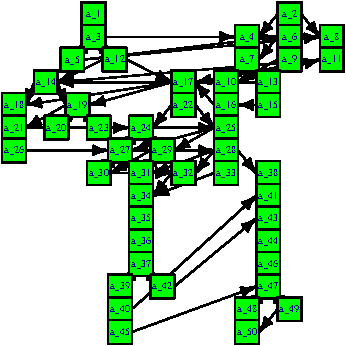
\includegraphics{AoN-1} }\subfloat[C2011-08 Sports Center Tielt logic (AoN) network\label{fig:AoN-2}]{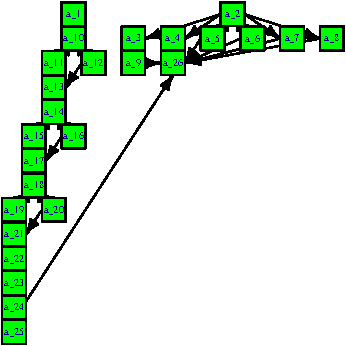
\includegraphics{AoN-2} }

}

\caption{Logical structures of synthetic (a) and real (b) project networks}\label{fig:AoN}
\end{figure}

The two project databases -- Boctor's synthetic dataset and Batselier
and Vanhoucke's real project dataset -- are worth choosing for
comparison because they provide complementary perspectives on project
network structures. Synthetic projects offer a controlled environment
with known completion modes and a randomized network properties, serving
as a baseline for understanding theoretical project scheduling
behaviors. In contrast, real projects reflect practical complexities,
constraints, and resource patterns encountered in actual project
management. Comparing these datasets reveals significant differences in
flexibility, efficiency, connectedness, and resilience, thereby
validating the utility of network-level indicators in distinguishing
real project characteristics from synthetic approximations. This
comparison enables the calibration and improvement of simulation models
and enhances project selection and prioritization methods that are on
the basis of more realistic network features. To further improve this
argument, one could explicitly highlight how the combined use of These
datasets help in identifying specific network-level indicators that are
robust and generalizable across both synthetic and real contexts, thus
reinforcing the empirical and practical relevance of the research
contributions. Further databases can be obtained from
\citet{kosztyan2024compound}.

\subsection{Applied methods and indicators}\label{subsec:methods}

The existing project indicators can be distinguished into three
clusters: (1) time-related indicators (see Section
\ref{subsubsec:timeindicators}), (2) (renewable) resource-related
indicators (see Section \ref{subsubsec:resindicators}), and structural
or logic indicators (see Section \ref{subsubsec:logicindicators}). The
proposed network indicators (see Section \ref{subsubsec:netindicators})
are closest to the structural indicators, but at the same time
complement them in many areas.

\subsubsection{Time-related indicators}\label{subsubsec:timeindicators}

The time-related indicators can be classified into three groups: (1)
\emph{Duration-related indicators}: These indicators measure the average
and the variance of the activity durations in a project. They include
average activity duration (XDUR) and variance in activity durations
(VADUR). These indicators are important because they help to estimate
the total project time, to identify the critical path, and to assess the
uncertainty and risk of the project schedule. (2-3) \emph{Slack-related
indicators} and \emph{Free-slack related indicators}: The slack-related
indicators measure the amount and the proportion of slack or float in a
project. Slack or float is the amount of time an activity can be delayed
without affecting the project completion date. These include number of
activities with positive (nonzero) total float (NSLACK), percentage of
activities with positive (nonzero) total float (PCTSLACK), total slack
ratio (TOTSLACK\_R), average slack (XSLACK), and average slack ratio
(XSLACK\_R). These measures are important because they indicate the
degree and the distribution of flexibility or buffer in the project
schedule, as well as the potential opportunities for resource leveling
or smoothing. The slack-free indicators measure the amount and the
proportion of free slack in a project. Free slack is the amount of time
an activity can be delayed without affecting the start of any other
activity in the project. These measures include number of activities
with positive (nonzero) free slack (NFREESLK), percentage of activities
with positive (nonzero) free slack (PCTFREESLK), and average free slack
(XFREESLK). They are important because they indicate the degree and the
distribution of flexibility or buffers for specific activities in the
project schedule, and potential opportunities for resource optimization
or reallocation.

\subsubsection{Resource-related
indicators}\label{subsubsec:resindicators}

These indicators measure the availability, demand, use, and efficiency
of renewable resources (such as labor, equipment, and materials) that
are needed to complete the project activities. They help to plan and
allocate the resources accordingly, to avoid resource shortages or
surpluses, optimizes resource utilization, and identifies resource
bottlenecks or gaps. These indicators can be classified into two groups.
(1) \emph{Availability and demand indicators}: These indicators measure
how many resources are available and how many resources are required for
the project activities. These include the number of renewable resources
(NRES), average resource demand (XDMND), percentage of activities
requiring positive amount of resource type (PCTR), resource strength
(RS), alpha distribution of resource strength (A\_RS), and normalized
average resource loading factor (NARLF). They help to assess the
resource feasibility and to identify the resource gaps for the earliest
start schedule, which minimizes the project duration and maximizes the
resource utilization. (2) \emph{Utilization and efficiency indicators}:
These indicators measure how the resources are used and how efficiently
they are used for project activities. These included resource use (RU),
average resource utilization (XUTIL), Gini coefficient (GINI), resource
constrainedness (for each resource type) (RC), average resource
constrainedness over time (XCON), resource factor (RF), total
obstruction factor (TOTOFACT) and total underutilization factor
(TOTUFACT). These variables help to evaluate resource efficiency and to
identify the resource bottlenecks or constraints that can cause delays
or inefficiencies in the project schedule. They also help to optimize
resource allocation by adjusting the resource demand or supply, by
levelling or smoothing the resources, by crashing or fast-tracking the
activities, or by changing the activity sequence or duration.

Another classification option is whether a schedule is needed to
calculate the indicator. (I) The \emph{nonscheduled resource-related
indicators} measure resource characteristics without considering the
project schedule or the activity start times. These include the NRES,
XDMND, RU, PCTR, GINI, RC, RF, and TOTOFACT. They provide a general
overview of the resource availability and demand, and the resource
distribution and diversity among the activities. (II) The
\emph{early-scheduled resource-related indicators} measure the resource
characteristics on the basis of the earliest start times of the
activities, which minimizes the project duration and maximizes resource
utilization. They include XUTIL, RS, A\_RS, NARLF, XCON, and TOTUFACT.
These measures provide a detailed analysis of resource feasibility and
efficiency as well as the resource gaps and bottlenecks for the earliest
start schedule.

\subsubsection{Logic indicators}\label{subsubsec:logicindicators}

Structural (logical) project indicators (see Table
\ref{tab:DESCLOGRELIND}) measure the complexity, flexibility, and the
interconnectedness of the project network. They help to understand the
logic and structure of the project, and how these factors affect the
project duration, risk, and resource allocation. The logic indicators
can be classified into two groups: (1) The \emph{complexity and
flexibility indicators} measure how complex and rigid or how simple and
flexible the project network is on the basis of the number and length of
the precedent relationships among the activities. These variables
include the serial-parallel (SP) indicator (I2), the length of long arcs
(LA) (I4), short arcs (SA) (I5), network complexity (C), coefficient of
network complexity (CNC), and order strength (OS). Such variables help
to assess the uncertainty and variability of the project schedule and
the potential opportunities for changing activities sequence or
duration. (2) \emph{Interconnectedness and robustness indicators}
measure how connected and robust the project network is, on the basis of
the number and degree of the nodes and the arcs in the network. These
variables include the activity distribution (AD) (I3), topological float
(TF) (I6), total activity density (TDENSITY), average activity density
(XDENSITY), number of articulation points (AP), components (COMPS),
degrees (MEAN\_DEGREE), and number of arcs (NARC). They help to evaluate
the impact and propagation of delays or disruptions in the project
schedule, and the potential opportunities for crashing or fast-tracking
activities.

The project network indicators provide a complementary perspective to
the logic indicator because the focus is on the network aspects of the
project, rather than on the objectives or the outputs. Despite
structural indicators already including several network parameters,
several important network-level measures are already missing.

\subsubsection{Network indicators}\label{subsubsec:netindicators}

Table \ref{tab:DESCNETRELIND} lists the proposed network-level
indicators when examining project networks. Like the logic indicators,
the proposed network indicators help to understand the logic and the
structure of the project and how they affect the project duration, risk,
and resource allocation. These indicators can be separated into seven
clusters. (1) The \emph{density and diameter indicators} measure how
many dependencies exist in the project network and how far apart the
tasks are in the network. They include Dens and Diam. These measures
indicate that the degree of complexity and dispersion of the project
network and how they influence the project schedule and resource
allocation. (2) \emph{Path length and asymmetry indicators} measure how
long and how uneven the paths are in the project network, on the basis
of the shortest distances between the tasks. They include AVPL and VAs.
These indices indicate the degree of concentration and diversity of the
project network and how they affect the project schedule and resources
allocation. (3) The \emph{motif and assortativity indicators} measure
how many recurring patterns and how similar the tasks are in the project
network, on the basis of the number and degree of dependencies. They
include the number of motifs (Mot) and assortativity (ASSORT). These
measures indicate the degree of regularity and the homogeneity of the
project network and how they influence the project schedule and resource
allocation. (4) \emph{Modularity and community indicators} measure how
well the project network can be partitioned into communities, on the
basis of different algorithms that optimize the modularity value. These
include Leiden's graph modularity value (LeM), Infomap's graph
modularity value (IM), and Spin-Glass graph modularity value SGM. These
measures of modularity and the community indicate the degree of
diversity and cohesion of the project network. Modularity can also help
to identify the subprojects or clusters of activities that have strong
dependencies within them but weak dependencies with other subprojects or
clusters. This can help to improve project management and coordination
by assigning different teams or resources to different subprojects or
clusters. (5) \emph{Centrality indicators} of how central or important
some tasks are in the project network, on the basis of different
criteria, such as degree, closeness, eigenvector, PageRank, and
betweenness. They also measure how centralized the network is as a
whole, on the basis of different indices such as alpha and power. They
include in-degree centralization (DZI), out-degree centralization (DZO),
degree centralization (DZ), closeness centralization (CZ), harmonic
centralization (HZ), eigenvector centralization (EZ), PageRank
centralization (PRZ), alpha centralization (AZ), power centralization
(PZ), betweenness centralization (BZ), and edge-betweenness
centralization (BEZ). These measures indicate the degree of dependency,
influence, accessibility, efficiency, importance, impact,
intermediation, and hierarchy of the tasks and the network. (6) The
\emph{resilience and efficiency indicators} measure how well the project
network can maintain its connectivity and efficiency when some tasks or
dependencies are removed, either randomly or systematically. These
variables include resilience for random attack (RRes), resilience for
systematic attack (SRes), average local efficiency (ALE), and global
efficiency (GE). They indicate the degree of robustness, susceptibility,
redundancy, and fragility of the project network. The role of indicators
is emphasized more in the case of agile projects where the task
completions must be prioritized \citep{CIRIC2019roleofflexibility}.
Because of the limited time and resource availability, several tasks
should be postponed to a later which can affect the change in the logic
structure of the project \citep{Kosztyan2015}. (7) Last but not least,
the \emph{transitivity indicator} measures how many triangles or closed
loops exist in the project network compared to the number of triplets or
open paths. It includes Tra. This measure is important because it
indicates the degree of cliquishness or openness of the project network.

\subsection{Applied supervised and unsupervised machine learning
algorithms}\label{subsec:algorithms}

To answer the research questions, first, descriptive statistics were
used to analyze synthetic and real-life project networks (see
\nameref{RQ1}). ANOVA revealed significant differences between real and
synthetic project plans are identified (see \nameref{RQ3}), and with
nongeneric approaches, such as the random forest method, variable
importance are also calculated (see Section \ref{subsubsec:supervised}).
To answer \nameref{RQ2}, \emph{traditional} methods, such as
hierarchical clustering and multidimensional scaling, and
\emph{nonparametric} unsupervised learning methods are applied to
identify groups of indicators, and the clusters of project networks (see
Section \ref{subsubsec:unsupervised}). These methods identify the
relationships between indicators and thier classification into indicator
groups (see \nameref{RQ2}). To maximize reproducibility by including the
source code of the entire article as supplementary material, which was
itself written in R, so that the entire calculation can be repeated.

\subsubsection{Descriptive statistics on standardized values and the
employed supervised learning methods}\label{subsubsec:supervised}

Prior to employing nongeneric techniques, such as the random forest (RF)
method, we utilized descriptive statistics and analysis of variance
(ANOVA) methodologies to investigate the project or network indicator
that exhibited the greatest disparity between real and synthetic
projects. To ensure a fair comparison, we standardized the variables in
the descriptive analysis. The unstandardized results are utilized in
ANOVA to determine the significance of differences.

In the case of ANOVA, in addition to \(R^2\) or adjusted \(R^2\), we
also calculates \(\eta^2\). The \(\eta^2\) measures of effect size or
variance explained by a factor or a variable in an ANOVA model. It is
different from \(R^2\) or adjusted \(R^2\), which are measures of
goodness of fit or how well the model predicts the outcome variable.

The employed supervised learning techniques can demonstrate how the
indicators are correlated with each other; therefore, instead of being
generic, such as logistic regression or linear discriminant analysis,
more robust nongeneric methods, such as the random forest (RF) method,
should be used to determine the importance of the variables. We split
our database at an 80-20 ratio, where 80\% was the training sample and
20\% was the test sample. We calculated the accuracy metrics, such as
accuracy, balanced accuracy, and F1-score on the test sample.

Since employed supervised learning techniques can show how the
indicators are correlated with each other; therefore, instead of being
generic, such as logistic regression or linear discriminant analysis,
more robust nongeneric methods, such as the random forest (RF) method,
should be used to identify the variable importance. Since we obtained
almost perfect accuracy both for logistic regression and the random
forest method, we did not use any other alternative solution.

\subsubsection{Employed unsupervised learning
methods}\label{subsubsec:unsupervised}

In addition to traditional clustering and dimensionality reduction
methods, such as hierarchical clustering and multidimensional scaling
techniques for detecting clusters of indicators and project networks, we
applied the generalized network-based dimensional reduction method
(GNDA) \citep{kosztyan2023network} instead of methods such as
nonnegative matrix factorization (NMF) \citep{saberi2024nonnegative} due
to GNDA's specific advantages in analyzing network structures. GNDA is
particularly suited for this research as it can handle both
high-dimensional low sample sizes (HDLSS) and low-dimensional high
sample sizes (LDHSS), offering greater flexibility and scalability in
analyzing diverse project network datasets.

The GNDA method has three mandatory (for dimensional and reduction) and
two supplementary steps (for feature selection). Since we applied this
method for feature selection, we use only the first three steps. Here,
we examined how the supervised clusters are separated from each other.

The GNDA algorithm initially computes the similarity graphs for either
the observations or the variables. The similarity function can be either
symmetrical, such as with correlation and Euclidean distance, or
asymmetric, such as with partial or semipartial correlations. The nodes
in this graph can be either observations or variables. Hence, this
approach can be employed for clustering either variables or
observations. In the second stage, modules are determined on the basis
of the similarity graph, where the density of connections between nodes
within the modules is greater than that of the nodes in different
modules. The community-based detection method is nonparametric, and
there is no require that the number of clusters be predefined. During
the third stage, the eigenvector centralities are computed for each
node. The latent variables for a module are computed as the product of
the standardized value of the data and the eigenvector centrality. This
process is analogous to principal component analysis However, in this
case, eigenvector centralities are defined as weights instead of
eigenvalues.

This method has several advantages over traditional unsupervised
machines learning techniques.

\begin{enumerate}
\def\labelenumi{\arabic{enumi}.}
\tightlist
\item
  \textbf{Scalability}. \citet{kosztyan2022network} reported that this
  method works not only on high-dimensional low sample sizes (HDLSS) but
  also on low-dimensional high sample sizes (LDHSS).
\item
  \textbf{Flexibility}. \citet{kosztyan2023network} reported that this
  technique can be used with various types of distance functions.
\item
  \textbf{Nonparametric}. There is no need to predefine the number of
  clusters or dimensions.
\end{enumerate}

The method calculates the NDA factor loadings, which are linear
combination of the eigenvector centrality of the indicator and the
standardized value of the given indicator. A larger factor absolute
value of the factor loadings indicates greater embeddedness in the
module and represents a greater influence on the latent variable.

Alternative techniques such as graph learning and spectral clustering
could potentially be applied to analyze project networks, as they are
well suited for capturing complex relationships in graph-structured data
\citep{berahmand2025comprehensive}. However, this study opts for
supervised and unsupervised learning methods, including random forest
and the GNDA, as they offer greater flexibility in handling both
network-level and project-specific indicators, and can effectively
address the research questions related to comparing real and synthetic
projects across multiple dimensions.

\subsection{Computational complexity}\label{sec:comcomplex}

The computational complexity of the methods employed in this study can
be grouped into three categories on the basis of their scalability for
large-scale projects:

\begin{enumerate}
\def\labelenumi{\arabic{enumi}.}
\item
  Linear complexity \(O(n)\) and quasilinear complexity \(O(n\log(n))\):
  Descriptive statistics, ANOVA, matrix representations and the
  calculation of most traditional and network-level indicators fall into
  this category, making them highly scalable for large datasets.
\item
  Polynomial complexity O(n\^{}k): Hierarchical clustering and
  multidimensional scaling techniques typically involve polynomial-time
  complexity, which may limit their scalability for very large projects.
\item
  Higher complexity: Random forest and generalized network-based
  dimensional reduction method (GNDA) generally results in higher
  computational complexity. The random forest has a time complexity of
  \(O(ntree \times nfeature \times nsamples \times \log(nsamples))\),
  where \(ntree\) is the number of trees and \(nfeature\) is the number
  of features, and nsamples is the number of samples. GNDA's complexity
  depends on the specific implementation but can be computationally
  intensive for large networks.
\end{enumerate}

For large-scale projects, methods in the first two categories would be
more readily applicable, whereas those in the third category might
require optimization or sampling techniques to maintain computational
feasibility.

\section{Results}\label{sec:results}

To address these resource questions, we compare the project and the
proposed network-level indicators. In Section \ref{subsec:descriptives},
we show the mean of standardized values of the project and network
indicators. In Section \ref{subsec:relind}, we show that a significant
relationship between the network and project (not only structural)
indicators. In Section \ref{subsec:simsynth}, we show that these
indicators can be used to classify project networks and can be used to
detect real and synthetic projects.

\subsection{Descriptive statistics}\label{subsec:descriptives}

Since the employed indicators can be interpreted at different intervals,
Table \ref{tab:MEANS_TIME} shows the standardized mean values of the
time-related indicators for synthetic and real projects.

\begin{table}[H]
\centering\centering
\caption{\label{tab:MEANS_TIME}Mean values of standardized time-related project indicators}
\centering
\fontsize{8}{10}\selectfont
\begin{tabular}[t]{lrrrrr}
\toprule
\multicolumn{1}{c}{ } & \multicolumn{4}{c}{Synthetic projects} & \multicolumn{1}{c}{ } \\
\cmidrule(l{3pt}r{3pt}){2-5}
\textbf{ } & \textbf{Mode 1} & \textbf{Mode 2} & \textbf{Mode 3} & \textbf{Mode 4} & \textbf{Real}\\
\midrule
\cellcolor{gray!10}{XDUR} & \cellcolor{gray!10}{-0.131} & \cellcolor{gray!10}{-0.102} & \cellcolor{gray!10}{-0.119} & \cellcolor{gray!10}{-0.203} & \cellcolor{gray!10}{1.880}\\
VADUR & -0.094 & -0.091 & -0.088 & -0.089 & 1.226\\
\cellcolor{gray!10}{MAXCPL} & \cellcolor{gray!10}{-0.173} & \cellcolor{gray!10}{-0.042} & \cellcolor{gray!10}{-0.057} & \cellcolor{gray!10}{-0.297} & \cellcolor{gray!10}{1.925}\\
NSLACK & 0.016 & 0.105 & 0.060 & -0.093 & -0.297\\
\cellcolor{gray!10}{PCTSLACK} & \cellcolor{gray!10}{0.014} & \cellcolor{gray!10}{0.259} & \cellcolor{gray!10}{0.116} & \cellcolor{gray!10}{-0.286} & \cellcolor{gray!10}{-0.347}\\
\addlinespace
TOTSLACK\_R & 0.090 & -0.215 & -0.209 & 0.594 & -0.877\\
\cellcolor{gray!10}{XSLACK} & \cellcolor{gray!10}{-0.159} & \cellcolor{gray!10}{-0.111} & \cellcolor{gray!10}{-0.104} & \cellcolor{gray!10}{-0.146} & \cellcolor{gray!10}{1.758}\\
XSLACK\_R & -0.270 & -0.205 & -0.129 & 0.041 & 1.906\\
\cellcolor{gray!10}{NFREESLK} & \cellcolor{gray!10}{0.290} & \cellcolor{gray!10}{0.305} & \cellcolor{gray!10}{0.157} & \cellcolor{gray!10}{-0.281} & \cellcolor{gray!10}{-1.591}\\
PCTFREESLK & 0.445 & 0.467 & 0.224 & -0.512 & -2.105\\
\addlinespace
\cellcolor{gray!10}{XFREESLK} & \cellcolor{gray!10}{-0.153} & \cellcolor{gray!10}{-0.029} & \cellcolor{gray!10}{-0.015} & \cellcolor{gray!10}{-0.148} & \cellcolor{gray!10}{1.164}\\
\bottomrule
\end{tabular}
\end{table}

The standardized values are calculated by subtracting the mean and
dividing by the standard deviation of the original values so that they
have a mean of zero and a standard deviation of one. This allows for a
fair comparison between different indicators and different projects.
Table \ref{tab:MEANS_TIME} shows the main differences between the
synthetic and real projects that are found in the following indicators:
(1) XDUR: The average activity duration is much greater for the real
projects than that for the synthetic projects, indicating that the real
projects have longer and more complex activities. (2) MAXCPL: The
maximum critical path length is also much greater for real projects than
that for the synthetic projects, indicating that the real projects have
longer and more constrained critical paths. (3) PCTSLACK and PCTFREESLK:
The percentage of activities with positive (nonzero) total slack and
free slack are much lower for real projects than that for synthetic
projects, indicating that real projects have increasingly less flexible
noncritical activities. (4) TOTSLACK\_R and XSLACK\_R: Total slack ratio
and the average slack ratio are much greater for real projects than
those for synthetic projects, indicating that real projects have more
slack per activity and per critical path length than does the synthetic
projects. (5) NFREESLK: The number of activities with positive (nonzero)
free slack is much lower for real projects than that for the synthetic
projects, indicating that real projects have fewer activities that can
be delayed without affecting the start of their successors.

Table \ref{tab:MEANS_RESOURCE} shows the standardized mean values of the
resource-related indicators for synthetic and real projects.

\begin{table}[H]
\centering\centering
\caption{\label{tab:MEANS_RESOURCE}Mean values of standardized resource-related project indicators}
\centering
\fontsize{8}{10}\selectfont
\begin{tabular}[t]{lrrrrr}
\toprule
\multicolumn{1}{c}{ } & \multicolumn{4}{c}{Synthetic projects} & \multicolumn{1}{c}{ } \\
\cmidrule(l{3pt}r{3pt}){2-5}
\textbf{ } & \textbf{Mode 1} & \textbf{Mode 2} & \textbf{Mode 3} & \textbf{Mode 4} & \textbf{Real}\\
\midrule
\cellcolor{gray!10}{NRES} & \cellcolor{gray!10}{-0.049} & \cellcolor{gray!10}{-0.049} & \cellcolor{gray!10}{-0.049} & \cellcolor{gray!10}{-0.049} & \cellcolor{gray!10}{0.660}\\
XDMND & -0.032 & -0.032 & -0.032 & -0.032 & 1.393\\
\cellcolor{gray!10}{RU} & \cellcolor{gray!10}{0.801} & \cellcolor{gray!10}{0.069} & \cellcolor{gray!10}{-0.141} & \cellcolor{gray!10}{-0.782} & \cellcolor{gray!10}{0.435}\\
XUTIL & 0.032 & 0.032 & 0.032 & 0.031 & -1.053\\
\cellcolor{gray!10}{PCTR} & \cellcolor{gray!10}{1.116} & \cellcolor{gray!10}{0.067} & \cellcolor{gray!10}{-0.017} & \cellcolor{gray!10}{-1.039} & \cellcolor{gray!10}{-1.047}\\
\addlinespace
RS & -0.682 & -0.419 & 0.102 & 1.375 & -0.489\\
\cellcolor{gray!10}{A\_RS} & \cellcolor{gray!10}{0.315} & \cellcolor{gray!10}{-0.028} & \cellcolor{gray!10}{0.162} & \cellcolor{gray!10}{-0.219} & \cellcolor{gray!10}{-0.778}\\
NARLF & -0.031 & -0.031 & -0.031 & -0.031 & 0.421\\
\cellcolor{gray!10}{GINI} & \cellcolor{gray!10}{-1.339} & \cellcolor{gray!10}{-0.180} & \cellcolor{gray!10}{0.285} & \cellcolor{gray!10}{1.238} & \cellcolor{gray!10}{-0.040}\\
RC & 0.032 & 0.032 & 0.032 & 0.032 & -1.392\\
\addlinespace
\cellcolor{gray!10}{XCON} & \cellcolor{gray!10}{0.032} & \cellcolor{gray!10}{0.032} & \cellcolor{gray!10}{0.032} & \cellcolor{gray!10}{0.032} & \cellcolor{gray!10}{-1.392}\\
RF & 0.946 & 0.239 & -0.047 & -1.074 & -0.531\\
\cellcolor{gray!10}{TOTOFACT} & \cellcolor{gray!10}{-0.024} & \cellcolor{gray!10}{-0.011} & \cellcolor{gray!10}{-0.066} & \cellcolor{gray!10}{-0.070} & \cellcolor{gray!10}{1.869}\\
TOTUFACT & -0.251 & -0.190 & 0.012 & 0.152 & 3.006\\
\bottomrule
\end{tabular}
\end{table}

The largest differences between synthetic and real projects are found in
the following indicators: (1) NRES: The number of renewable resources is
much greater for real projects than for synthetic projects, indicating
that real projects have more types of resources available for scheduling
activities. (2) XDMND: The average resource demand is much greater for
real projects than for synthetic projects, indicating that real projects
have more resource requirements for each activity. (3) RU: the resource
use varies more for synthetic projects than that for real projects,
which indicates that the synthetic projects have different degrees of
resource diversity among the activities. (4) XUTIL: The average resource
utilization is much lower for real projects than that for synthetic
projects, indicating that real projects have lower resource efficiency
and higher resource bottlenecks on the longest critical path. (5) PCTR:
The percentage of activities requiring a positive amount of resource
type is much lower for real projects than that for synthetic projects,
indicating that real projects have fewer resources distribution and more
resource concentration among the activities. (6) RS: The resource
strength is more variable for synthetic projects than that for real
projects, indicating that synthetic projects have different degrees of
resource feasibility and resource gaps for the earliest start schedule
of each activity. (7) A\_RS: The alpha distribution of resource strength
is much lower for real projects than that for the synthetic projects,
indicating that the real projects have less variation in resource
strengths across different subprojects or disconnected components in the
project network. (8) GINI: The Gini coefficient is more variable for
synthetic projects than for real projects, indicating that the synthetic
projects have different degrees of resource inequality or diversity
among activities. (9) RC and XCON: The resource constraint (for each
resource type and over time) is much lower for real projects than for
synthetic projects, indicating that real projects have less resource
tightness or scarcity for each resource type and over time. (10) RF: The
resource factor is more variable for synthetic projects than for real
projects, indicating that the synthetic projects have different degrees
of resource density or complexity in the resource matrix. (11) TOTOFACT
and TOTUFACT: Total obstruction factor and total underutilization
factors are much greater for real projects than those for the synthetic
projects, indicating that the real projects have more excessive and
underutilized resource needs for the earliest start schedule.

Table \ref{tab:MEANS_LOGIC} shows the standardized mean values of the
structural (logic) and network indicators for synthetic and real
projects.

\begin{table}[H]
\centering
\caption{\label{tab:MEANS_LOGIC}Mean values of standardized structural (logic) and network indicators}
\begin{minipage}{0.48\linewidth}
\begingroup\fontsize{8}{10}\selectfont

\begin{tabular}{lrr}
\toprule
\textbf{ } & \textbf{Synthetic} & \textbf{Real}\\
\midrule
\cellcolor{gray!10}{TASKS} & \cellcolor{gray!10}{0.055} & \cellcolor{gray!10}{-0.745}\\
I2 & 0.002 & -0.026\\
\cellcolor{gray!10}{I3} & \cellcolor{gray!10}{-0.126} & \cellcolor{gray!10}{1.700}\\
I4 & -0.048 & 0.655\\
\cellcolor{gray!10}{I5} & \cellcolor{gray!10}{0.016} & \cellcolor{gray!10}{-0.215}\\
\addlinespace
I6 & -0.173 & 2.338\\
\cellcolor{gray!10}{C} & \cellcolor{gray!10}{0.111} & \cellcolor{gray!10}{-1.497}\\
CNC & 0.179 & -2.420\\
\cellcolor{gray!10}{OS} & \cellcolor{gray!10}{0.170} & \cellcolor{gray!10}{-2.303}\\
TDENSITY & 0.057 & -0.773\\
\addlinespace
\cellcolor{gray!10}{XDENSITY} & \cellcolor{gray!10}{0.025} & \cellcolor{gray!10}{-0.345}\\
AP & -0.131 & 1.772\\
\cellcolor{gray!10}{COMPS} & \cellcolor{gray!10}{-0.054} & \cellcolor{gray!10}{0.732}\\
MEAN\_DEGREE & 0.179 & -2.420\\
\cellcolor{gray!10}{NARC} & \cellcolor{gray!10}{0.083} & \cellcolor{gray!10}{-1.126}\\
\bottomrule
\multicolumn{3}{l}{\rule{0pt}{1em}(a) logic indicators}\\
\end{tabular}
\endgroup{}
\end{minipage}\quad
\begin{minipage}{0.48\linewidth}
\begingroup\fontsize{8}{10}\selectfont

\begin{tabular}{lrr}
\toprule
\textbf{\textbf{ }} & \textbf{\textbf{Synthetic}} & \textbf{\textbf{Real}}\\
\midrule
\cellcolor{gray!10}{Dens} & \cellcolor{gray!10}{-0.123} & \cellcolor{gray!10}{1.667}\\
Diam & 0.015 & -0.201\\
\cellcolor{gray!10}{AVPL} & \cellcolor{gray!10}{0.028} & \cellcolor{gray!10}{-0.374}\\
VAs & -0.065 & 0.878\\
\cellcolor{gray!10}{Mot} & \cellcolor{gray!10}{0.062} & \cellcolor{gray!10}{-0.832}\\
\addlinespace
ASSORT & -0.037 & 0.495\\
\cellcolor{gray!10}{LeM} & \cellcolor{gray!10}{0.046} & \cellcolor{gray!10}{-0.623}\\
IM & 0.069 & -0.936\\
\cellcolor{gray!10}{SGM} & \cellcolor{gray!10}{0.051} & \cellcolor{gray!10}{-0.685}\\
DZI & -0.081 & 1.089\\
\addlinespace
\cellcolor{gray!10}{DZO} & \cellcolor{gray!10}{-0.156} & \cellcolor{gray!10}{2.107}\\
DZ & -0.121 & 1.639\\
\cellcolor{gray!10}{CZ} & \cellcolor{gray!10}{-0.064} & \cellcolor{gray!10}{0.872}\\
HZ & -0.002 & 0.028\\
\cellcolor{gray!10}{EZ} & \cellcolor{gray!10}{0.030} & \cellcolor{gray!10}{-0.412}\\
\addlinespace
PRZ & 0.024 & -0.322\\
\cellcolor{gray!10}{AZ} & \cellcolor{gray!10}{0.031} & \cellcolor{gray!10}{-0.416}\\
PZ & 0.067 & -0.906\\
\cellcolor{gray!10}{BZ} & \cellcolor{gray!10}{0.040} & \cellcolor{gray!10}{-0.541}\\
BEZ & -0.018 & 0.245\\
\addlinespace
\cellcolor{gray!10}{RRes} & \cellcolor{gray!10}{0.083} & \cellcolor{gray!10}{-1.123}\\
SRes & 0.099 & -1.341\\
\cellcolor{gray!10}{ALE} & \cellcolor{gray!10}{0.104} & \cellcolor{gray!10}{-1.408}\\
GE & -0.042 & 0.565\\
\cellcolor{gray!10}{Tra} & \cellcolor{gray!10}{-0.093} & \cellcolor{gray!10}{1.256}\\
\bottomrule
\multicolumn{3}{l}{\rule{0pt}{1em}(b) network indicators}\\
\end{tabular}
\endgroup{}
\end{minipage}
\end{table}

The largest differences between synthetic and real projects are found in
the following logic and network indicators: (1) Dens: The density is
much greater for real projects than that for synthetic projects,
indicating that real projects have more arcs per node and more
connections between the activities. (2) I3: The activity distribution is
much greater for real projects than that for synthetic projects,
indicating that the real projects have more balanced and evenly
distributed activities. (3) DZO: The out-degree centralization is much
higher for real projects than that for synthetic projects, indicating
that the real projects have more variation in the number of successors
per activity or more activities with many successors. (4) C and CNC: The
network complexity and the coefficient of network complexity are much
lower for real projects than those for synthetic projects, indicating
that real projects have simpler and less dense project networks. (5) OS:
The order strength is much lower for the real projects than that for the
synthetic projects, indicating that the real projects have fewer
constrained and more flexible project networks. (6) AP and COMPS: The
number of articulation points and components are greater for real
projects than those for synthetic projects, indicating that real
projects have more disconnected and modular project networks. (7) SRes:
The resilience to systematic attack is much lower for real projects than
for synthetic projects, indicating that real projects are more
vulnerable to targeted disruptions of activities. (8) Tra: The graph
transitivity is much greater for real projects than for synthetic
projects, indicating that real projects have more triangles and more
clustering of the activities.

Tables \ref{tab:MEANS_TIME}-\ref{tab:MEANS_LOGIC} show that both project
and network indicators greatly differ between synthetic and real project
datasets. Figure \ref{fig:MDS}(a) shows that the distance between
project and network indicators via multidimensional scaling and Figure
\ref{fig:MDS}(b) shows the results of hierarchical clustering of the
project networks.

\begin{figure}[H]

{\centering \subfloat[Multidimensional scaling\label{fig:MDS-1}]{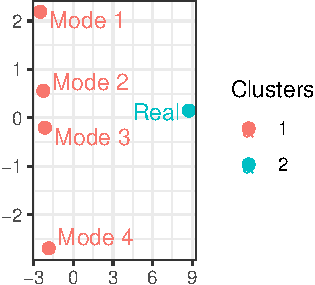
\includegraphics{MDS-1} }\subfloat[Dendogram of hierarchical clustering\label{fig:MDS-2}]{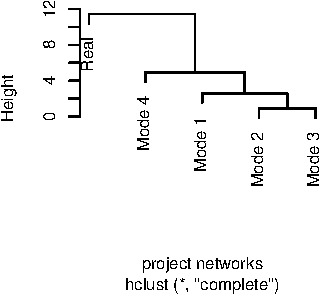
\includegraphics{MDS-2} }

}

\caption{Comparison of real and synthetic datasets on the basis of project and network indicators}\label{fig:MDS}
\end{figure}

Figure \ref{fig:MDS}(a) shows that for the vertical factor and the
completion modes also differ. However, these differences are much less
than those differences between real and synthetic projects, which is
also confirmed by the results of hierarchical clustering (see Figure
\ref{fig:MDS}(b)). The silhouette measure is: 60.31\%, which indicates a
fair classification. Nevertheless, Tables
\ref{tab:MEANS_TIME}-\ref{tab:MEANS_LOGIC} show that distances between
real and synthetic projects are significant both for project and network
indicators. The largest distance of the project indicators occurs if we
compare the real project with completion mode 1 synthetic project
networks. Since real and synthetic project plans are significantly
separated in the indicators, it is possible to classify project plans by
using the data. The classification also reveals which indicator (or
indicator groups) is the one that separates real and synthetic projects
(see Section \ref{subsec:simsynth}).

\subsection{Relationship between project and network
indicators}\label{subsec:relind}

Figure \ref{fig:NDA_FIG} shows the correlation graph of the project and
the network indicators. In the correlation network, the vertices are the
indicators, the edges are the correlation relationships between the
variables. The thicker an edge is, the closer the connection between
them is. The size of the nodes is proportional to the number of
correlations. By using the Force Atlas II \citep{Jacomy2014ForceAtlas2}
algorithm, vertices with many connections are located in the center of
the network, whereas vertices with few connections are located on the
periphery of the network. The colors depend on which indicator belongs
to which module. The connections between modules are given the same
color. Indicators marked in black do not belong to any module.

\begin{figure}[H]

{\centering 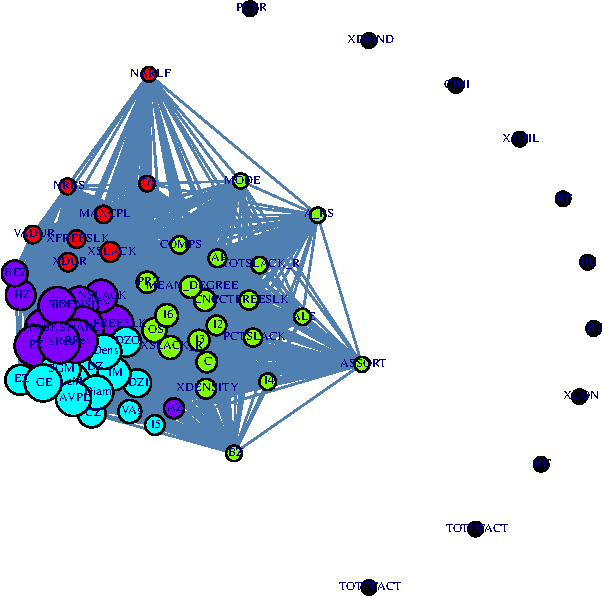
\includegraphics{NDA_FIG-1} 

}

\caption{Clustered correlation graph of the project and network indicators}\label{fig:NDA_FIG}
\end{figure}

The employed NDA method identifies four clusters. This method also
calculates the factor loading values of these indicators, which is a
linear combination of their eigenvector centralities and the values of
latent variables. A higher absolute value of the factor loadings
indicates grater embeddedness in the module. Table \ref{tab:NDA_TOP5}
shows the top five indicators which are ranked by the decreasing
absolute values of the factor loadings, while the following indicators
do not belong to any module: RU, PCTR, RS, GINI, RC, RF, TOTOFACT,
TOTUFACT, XCON, XDMND, XUTIL, which we considered as outliers.

\begin{table}
\centering
\caption{\label{tab:NDA_TOP5}Top 5 indicators and their NDA factor loadings values}
\centering
\begin{tabular}[t]{lrlrlrlr}
\toprule
\textbf{VAR1} & \textbf{NDA1} & \textbf{VAR2} & \textbf{NDA2} & \textbf{VAR3} & \textbf{NDA3} & \textbf{VAR4} & \textbf{NDA4}\\
\midrule
AP & 0.964 & Diam & 0.998 & AZ & 1.000 & VADUR & 1.000\\
COMPS & 0.797 & AVPL & 0.989 & NFREESLK & 0.472 & XDUR & 0.820\\
XSLACK\_R & 0.521 & LeM & 0.834 & NARC & 0.422 & XFREESLK & 0.791\\
OS & -0.500 & SGM & 0.833 & RRes & 0.379 & XSLACK & 0.760\\
I6 & 0.498 & GE & -0.772 & TASKS & 0.365 & MAXCPL & 0.718\\
\bottomrule
\end{tabular}
\end{table}

Table \ref{tab:NDA_TOP5} shows that in three of the four clusters, the
structural and network-level indicators are dominant, whereas the fourth
cluster mainly collects time-dependent indicators. Table
\ref{tab:PDF_MTX} shows the relative frequencies of the indicator groups
in clusters, where cluster zero collects the outliers (mainly resource
indicators).

\begin{table}[H]
\centering
\caption{\label{tab:PDF_MTX}Percentage distribution of different project and network indicator types}
\centering
\begin{tabular}[t]{lrrrrr}
\toprule
\textbf{ } & \textbf{Cluster\_0} & \textbf{Cluster\_1} & \textbf{Cluster\_2} & \textbf{Cluster\_3} & \textbf{Cluster\_4}\\
\midrule
\cellcolor{gray!10}{Time} & \cellcolor{gray!10}{0.00\%} & \cellcolor{gray!10}{36.36\%} & \cellcolor{gray!10}{0.00\%} & \cellcolor{gray!10}{18.18\%} & \cellcolor{gray!10}{45.45\%}\\
Resource & 78.57\% & 7.14\% & 0.00\% & 0.00\% & 14.29\%\\
\cellcolor{gray!10}{Logic} & \cellcolor{gray!10}{0.00\%} & \cellcolor{gray!10}{73.33\%} & \cellcolor{gray!10}{6.67\%} & \cellcolor{gray!10}{20.00\%} & \cellcolor{gray!10}{0.00\%}\\
Network & 0.00\% & 16.00\% & 52.00\% & 28.00\% & 4.00\%\\
\bottomrule
\end{tabular}
\end{table}

\subsection{Similarities and differences between synthetic and real
project networks}\label{subsec:simsynth}

In this section, we employed the analysis of variance approach to
determine the variables that exhibit significant differences between the
systematic and real datasets (see Section \ref{subsubsec:ANOVA}).
Additionally, we utilized the random forest method to compute the
importance of each variable (see Section \ref{subsubsec:RF}).

\subsubsection{Analyis of variances}\label{subsubsec:ANOVA}

Table \ref{tab:ANOVA} shows which indicators are significantly different
in the case of synthetic project networks.

\begingroup\fontsize{8}{10}\selectfont

\begin{longtable}[t]{llrrrrrl}
\caption{\label{tab:ANOVA}Analysis of variance for detecting the difference in indicators between synthetic and real project networks}\\
\toprule
\textbf{ } & \textbf{Type} & \textbf{Df} & \textbf{Sum Sq} & \textbf{Mean Sq} & \textbf{F value} & \textbf{Pr($<$F)} & \textbf{Sig.}\\
\midrule
\endfirsthead
\caption[]{Analysis of variance for detecting the difference in indicators between synthetic and real project networks \textit{(continued)}}\\
\toprule
\textbf{ } & \textbf{Type} & \textbf{Df} & \textbf{Sum Sq} & \textbf{Mean Sq} & \textbf{F value} & \textbf{Pr($<$F)} & \textbf{Sig.}\\
\midrule
\endhead

\endfoot
\bottomrule
\multicolumn{8}{l}{\rule{0pt}{1em}\textit{Note: }}\\
\multicolumn{8}{l}{\rule{0pt}{1em}$\sum \eta^2$ = 0.969, $R^2$ = 0.969, Adj. $R^2$ = 0.962}\\
\multicolumn{8}{l}{\rule{0pt}{1em}Sum of squares (Sq) are calcultated by type II mode}\\
\multicolumn{8}{l}{\rule{0pt}{1em}Signif. codes:  0 '***' 0.001 '**' 0.01 '*' 0.05 '.' 0.1 ' ' 1}\\
\endlastfoot
\cellcolor{gray!10}{XDUR} & \cellcolor{gray!10}{Time} & \cellcolor{gray!10}{1} & \cellcolor{gray!10}{12.385} & \cellcolor{gray!10}{12.385} & \cellcolor{gray!10}{1859.092} & \cellcolor{gray!10}{0.000} & \cellcolor{gray!10}{***}\\
VADUR & Time & 1 & 0.984 & 0.984 & 147.730 & 0.000 & ***\\
\cellcolor{gray!10}{MAXCPL} & \cellcolor{gray!10}{Time} & \cellcolor{gray!10}{1} & \cellcolor{gray!10}{4.143} & \cellcolor{gray!10}{4.143} & \cellcolor{gray!10}{621.854} & \cellcolor{gray!10}{0.000} & \cellcolor{gray!10}{***}\\
NSLACK & Time & 1 & 0.237 & 0.237 & 35.522 & 0.000 & ***\\
\cellcolor{gray!10}{PCTSLACK} & \cellcolor{gray!10}{Time} & \cellcolor{gray!10}{1} & \cellcolor{gray!10}{0.020} & \cellcolor{gray!10}{0.020} & \cellcolor{gray!10}{3.010} & \cellcolor{gray!10}{0.084} & \cellcolor{gray!10}{.}\\
\addlinespace
TOTSLACK R & Time & 1 & 0.231 & 0.231 & 34.656 & 0.000 & ***\\
\cellcolor{gray!10}{XSLACK} & \cellcolor{gray!10}{Time} & \cellcolor{gray!10}{1} & \cellcolor{gray!10}{10.460} & \cellcolor{gray!10}{10.460} & \cellcolor{gray!10}{1570.110} & \cellcolor{gray!10}{0.000} & \cellcolor{gray!10}{***}\\
XSLACK R & Time & 1 & 12.800 & 12.800 & 1921.302 & 0.000 & ***\\
\cellcolor{gray!10}{NFREESLK} & \cellcolor{gray!10}{Time} & \cellcolor{gray!10}{1} & \cellcolor{gray!10}{1.254} & \cellcolor{gray!10}{1.254} & \cellcolor{gray!10}{188.300} & \cellcolor{gray!10}{0.000} & \cellcolor{gray!10}{***}\\
PCTFREESLK & Time & 1 & 2.188 & 2.188 & 328.494 & 0.000 & ***\\
\addlinespace
\cellcolor{gray!10}{XFREESLK} & \cellcolor{gray!10}{Time} & \cellcolor{gray!10}{1} & \cellcolor{gray!10}{0.151} & \cellcolor{gray!10}{0.151} & \cellcolor{gray!10}{22.727} & \cellcolor{gray!10}{0.000} & \cellcolor{gray!10}{***}\\
NRES & Resource & 1 & 0.061 & 0.061 & 9.195 & 0.003 & **\\
\cellcolor{gray!10}{A RS} & \cellcolor{gray!10}{Resource} & \cellcolor{gray!10}{1} & \cellcolor{gray!10}{0.367} & \cellcolor{gray!10}{0.367} & \cellcolor{gray!10}{55.057} & \cellcolor{gray!10}{0.000} & \cellcolor{gray!10}{***}\\
NARLF & Resource & 1 & 0.007 & 0.007 & 1.111 & 0.293 & \\
\cellcolor{gray!10}{TASKS} & \cellcolor{gray!10}{Logic} & \cellcolor{gray!10}{1} & \cellcolor{gray!10}{0.495} & \cellcolor{gray!10}{0.495} & \cellcolor{gray!10}{74.347} & \cellcolor{gray!10}{0.000} & \cellcolor{gray!10}{***}\\
\addlinespace
I2 & Logic & 1 & 0.688 & 0.688 & 103.278 & 0.000 & ***\\
\cellcolor{gray!10}{I3} & \cellcolor{gray!10}{Logic} & \cellcolor{gray!10}{1} & \cellcolor{gray!10}{1.424} & \cellcolor{gray!10}{1.424} & \cellcolor{gray!10}{213.805} & \cellcolor{gray!10}{0.000} & \cellcolor{gray!10}{***}\\
I4 & Logic & 1 & 0.557 & 0.557 & 83.639 & 0.000 & ***\\
\cellcolor{gray!10}{I5} & \cellcolor{gray!10}{Logic} & \cellcolor{gray!10}{1} & \cellcolor{gray!10}{0.110} & \cellcolor{gray!10}{0.110} & \cellcolor{gray!10}{16.534} & \cellcolor{gray!10}{0.000} & \cellcolor{gray!10}{***}\\
I6 & Logic & 1 & 0.015 & 0.015 & 2.229 & 0.137 & \\
\addlinespace
\cellcolor{gray!10}{C} & \cellcolor{gray!10}{Logic} & \cellcolor{gray!10}{1} & \cellcolor{gray!10}{0.002} & \cellcolor{gray!10}{0.002} & \cellcolor{gray!10}{0.344} & \cellcolor{gray!10}{0.558} & \cellcolor{gray!10}{}\\
CNC & Logic & 1 & 0.295 & 0.295 & 44.293 & 0.000 & ***\\
\cellcolor{gray!10}{OS} & \cellcolor{gray!10}{Logic} & \cellcolor{gray!10}{1} & \cellcolor{gray!10}{1.094} & \cellcolor{gray!10}{1.094} & \cellcolor{gray!10}{164.246} & \cellcolor{gray!10}{0.000} & \cellcolor{gray!10}{***}\\
TDENSITY & Logic & 1 & 0.128 & 0.128 & 19.257 & 0.000 & ***\\
\cellcolor{gray!10}{XDENSITY} & \cellcolor{gray!10}{Logic} & \cellcolor{gray!10}{1} & \cellcolor{gray!10}{0.218} & \cellcolor{gray!10}{0.218} & \cellcolor{gray!10}{32.724} & \cellcolor{gray!10}{0.000} & \cellcolor{gray!10}{***}\\
\addlinespace
AP & Logic & 1 & 0.011 & 0.011 & 1.604 & 0.206 & \\
\cellcolor{gray!10}{COMPS} & \cellcolor{gray!10}{Logic} & \cellcolor{gray!10}{1} & \cellcolor{gray!10}{0.009} & \cellcolor{gray!10}{0.009} & \cellcolor{gray!10}{1.334} & \cellcolor{gray!10}{0.249} & \cellcolor{gray!10}{}\\
MEAN DEGREE & Logic & 1 & 0.199 & 0.199 & 29.878 & 0.000 & ***\\
\cellcolor{gray!10}{NARC} & \cellcolor{gray!10}{Logic} & \cellcolor{gray!10}{1} & \cellcolor{gray!10}{0.020} & \cellcolor{gray!10}{0.020} & \cellcolor{gray!10}{2.979} & \cellcolor{gray!10}{0.086} & \cellcolor{gray!10}{.}\\
Dens & Network & 1 & 0.015 & 0.015 & 2.256 & 0.134 & \\
\addlinespace
\cellcolor{gray!10}{Diam} & \cellcolor{gray!10}{Network} & \cellcolor{gray!10}{1} & \cellcolor{gray!10}{0.137} & \cellcolor{gray!10}{0.137} & \cellcolor{gray!10}{20.527} & \cellcolor{gray!10}{0.000} & \cellcolor{gray!10}{***}\\
AVPL & Network & 1 & 0.000 & 0.000 & 0.065 & 0.798 & \\
\cellcolor{gray!10}{VAs} & \cellcolor{gray!10}{Network} & \cellcolor{gray!10}{1} & \cellcolor{gray!10}{0.018} & \cellcolor{gray!10}{0.018} & \cellcolor{gray!10}{2.643} & \cellcolor{gray!10}{0.105} & \cellcolor{gray!10}{}\\
Mot & Network & 1 & 0.268 & 0.268 & 40.254 & 0.000 & ***\\
\cellcolor{gray!10}{ASSORT} & \cellcolor{gray!10}{Network} & \cellcolor{gray!10}{1} & \cellcolor{gray!10}{0.263} & \cellcolor{gray!10}{0.263} & \cellcolor{gray!10}{39.416} & \cellcolor{gray!10}{0.000} & \cellcolor{gray!10}{***}\\
\addlinespace
LeM & Network & 1 & 0.237 & 0.237 & 35.649 & 0.000 & ***\\
\cellcolor{gray!10}{IM} & \cellcolor{gray!10}{Network} & \cellcolor{gray!10}{1} & \cellcolor{gray!10}{0.200} & \cellcolor{gray!10}{0.200} & \cellcolor{gray!10}{29.952} & \cellcolor{gray!10}{0.000} & \cellcolor{gray!10}{***}\\
SGM & Network & 1 & 0.015 & 0.015 & 2.184 & 0.141 & \\
\cellcolor{gray!10}{DZI} & \cellcolor{gray!10}{Network} & \cellcolor{gray!10}{1} & \cellcolor{gray!10}{0.031} & \cellcolor{gray!10}{0.031} & \cellcolor{gray!10}{4.597} & \cellcolor{gray!10}{0.033} & \cellcolor{gray!10}{*}\\
DZO & Network & 1 & 0.003 & 0.003 & 0.484 & 0.487 & \\
\addlinespace
\cellcolor{gray!10}{DZ} & \cellcolor{gray!10}{Network} & \cellcolor{gray!10}{1} & \cellcolor{gray!10}{0.160} & \cellcolor{gray!10}{0.160} & \cellcolor{gray!10}{24.010} & \cellcolor{gray!10}{0.000} & \cellcolor{gray!10}{***}\\
CZ & Network & 1 & 0.076 & 0.076 & 11.337 & 0.001 & ***\\
\cellcolor{gray!10}{HZ} & \cellcolor{gray!10}{Network} & \cellcolor{gray!10}{1} & \cellcolor{gray!10}{0.133} & \cellcolor{gray!10}{0.133} & \cellcolor{gray!10}{19.942} & \cellcolor{gray!10}{0.000} & \cellcolor{gray!10}{***}\\
EZ & Network & 1 & 0.049 & 0.049 & 7.323 & 0.007 & **\\
\cellcolor{gray!10}{PRZ} & \cellcolor{gray!10}{Network} & \cellcolor{gray!10}{1} & \cellcolor{gray!10}{0.003} & \cellcolor{gray!10}{0.003} & \cellcolor{gray!10}{0.385} & \cellcolor{gray!10}{0.536} & \cellcolor{gray!10}{}\\
\addlinespace
AZ & Network & 1 & 0.004 & 0.004 & 0.565 & 0.453 & \\
\cellcolor{gray!10}{PZ} & \cellcolor{gray!10}{Network} & \cellcolor{gray!10}{1} & \cellcolor{gray!10}{0.005} & \cellcolor{gray!10}{0.005} & \cellcolor{gray!10}{0.737} & \cellcolor{gray!10}{0.391} & \cellcolor{gray!10}{}\\
BZ & Network & 1 & 0.409 & 0.409 & 61.346 & 0.000 & ***\\
\cellcolor{gray!10}{BEZ} & \cellcolor{gray!10}{Network} & \cellcolor{gray!10}{1} & \cellcolor{gray!10}{0.092} & \cellcolor{gray!10}{0.092} & \cellcolor{gray!10}{13.754} & \cellcolor{gray!10}{0.000} & \cellcolor{gray!10}{***}\\
RRes & Network & 1 & 0.087 & 0.087 & 13.129 & 0.000 & ***\\
\addlinespace
\cellcolor{gray!10}{SRes} & \cellcolor{gray!10}{Network} & \cellcolor{gray!10}{1} & \cellcolor{gray!10}{0.013} & \cellcolor{gray!10}{0.013} & \cellcolor{gray!10}{2.016} & \cellcolor{gray!10}{0.157} & \cellcolor{gray!10}{}\\
ALE & Network & 1 & 0.047 & 0.047 & 7.037 & 0.008 & **\\
\cellcolor{gray!10}{GE} & \cellcolor{gray!10}{Network} & \cellcolor{gray!10}{1} & \cellcolor{gray!10}{0.004} & \cellcolor{gray!10}{0.004} & \cellcolor{gray!10}{0.553} & \cellcolor{gray!10}{0.458} & \cellcolor{gray!10}{}\\
Tra & Network & 1 & 0.264 & 0.264 & 39.578 & 0.000 & ***\\
\midrule*
\end{longtable}
\endgroup{}

The independent variables are grouped into four types: time, resource,
logic, and network. These types represent different aspects of the
project network indicators, such as duration, resource allocation,
network structure, and network properties. The dependent variable is
whether a project network is synthetic or real, which means whether it
was generated via a simulation model or derived from a real project.

Table \ref{tab:ANOVA} shows that most of the projects (time, resources,
logic), and the network indicators are significant at the \(p=0.05\)
level. In addition, the variance explained is (\(\sum \eta^2\) = 96.9\%)
acceptable, and the goodness of fit values are (\(R^2\) = 96.9\%, Adj.
\(R^2\) = 96.2\%) also high.

\subsubsection{Calculating relative importances with random forest
methods}\label{subsubsec:RF}

Table \ref{tab:ANOVA} shows that most project and network indicators are
significant. However, the independent variables can have nonlinear
connections. Therefore, we used the Boruta \citep{Borutapkg} method to
(a) identify significant variables, and afterward, with a random forest
method, (2) we rank the indicators by their variable importance.

After Boruta was calculated only the following indicators: number of
renewable resources (NRES), number of articulation points (AP) are
removed from the model. Figure \ref{fig:Boruta} shows the variable
importance obtained via a tuned random forest method.

\begin{figure}[H]

{\centering 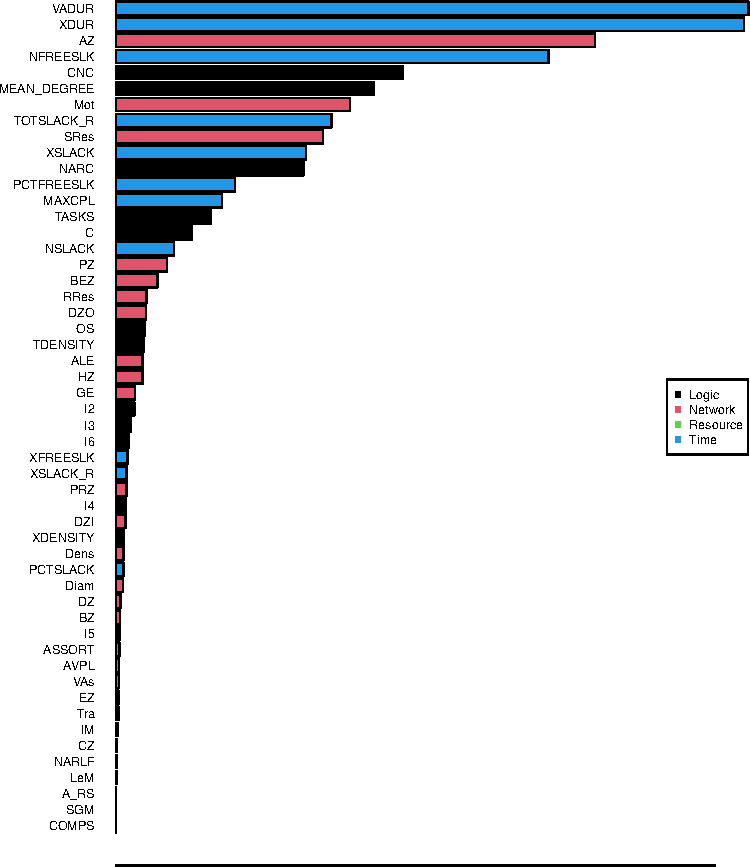
\includegraphics{Boruta-1} 

}

\caption{Ranked indicators by variable importance via the tuned random forest method}\label{fig:Boruta}
\end{figure}

Table \ref{tab:ACCURACY} shows the most important accuracy measures.

\begingroup\fontsize{8}{10}\selectfont

\begin{longtable}[t]{lrrrr}
\caption{\label{tab:ACCURACY}Accuracy measures of logistic regression and random forest methods}\\
\toprule
\textbf{ } & \textbf{Accuracy} & \textbf{AccuracyPValue} & \textbf{Balanced Accuracy} & \textbf{F1}\\
\midrule
\endfirsthead
\caption[]{Accuracy measures of logistic regression and random forest methods \textit{(continued)}}\\
\toprule
\textbf{ } & \textbf{Accuracy} & \textbf{AccuracyPValue} & \textbf{Balanced Accuracy} & \textbf{F1}\\
\midrule
\endhead

\endfoot
\bottomrule
\endlastfoot
Logistic Reg. & 0.98039 & 6e-05 & 0.95455 & 0.95238\\
Random Forest & 1.00000 & 0e+00 & 1.00000 & 1.00000\\*
\end{longtable}
\endgroup{}

The accuracy of both the logistic regression and the random forest
method is high. The first three indicators: variance in activity
durations (VADUR), and average activity duration (XDUR) are time-related
indicators. However, the third most important indicator for identifying
the separation between synthetic and real project networks is a network
indicator: alpha centralization (AZ).

\subsection{Unsupervised learning methods for identifying project
networks}\label{unsupervised-learning-methods-for-identifying-project-networks}

Figure \ref{fig:NDA_SYNPROJ} shows how the indicators are separated into
four-four clusters by using the GNDA method. Figure
\ref{fig:NDA_SYNPROJ}(a) (Figure \ref{fig:NDA_SYNPROJ}(b)) shows the
clustering results for only synthetic (only real) project networks are
considered.

\begin{figure}[H]

{\centering \subfloat[Synthetic data\label{fig:NDA_SYNPROJ-1}]{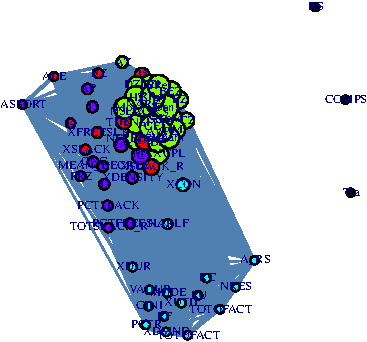
\includegraphics{NDA_SYNPROJ-1} }\subfloat[Real data\label{fig:NDA_SYNPROJ-2}]{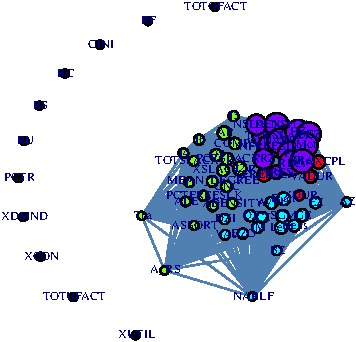
\includegraphics{NDA_SYNPROJ-2} }

}

\caption{Clustered correlation graph of the project and network indicators on synthetic and real project databases}\label{fig:NDA_SYNPROJ}
\end{figure}

Figure \ref{fig:NDA_DISTS} shows the clustered project networks if only
the proposed network indicators (see Figure \ref{fig:NDA_DISTS}(a)) or
the project indicators are employed (see Figure \ref{fig:NDA_DISTS}(b)).

\begin{figure}[H]

{\centering \subfloat[Only network indicators\label{fig:NDA_DISTS-1}]{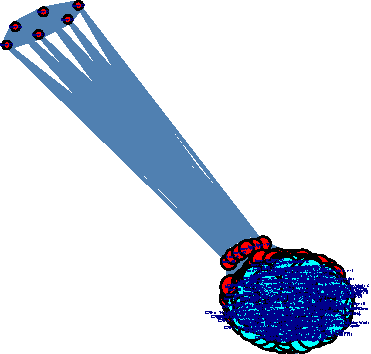
\includegraphics{NDA_DISTS-1} }\subfloat[Project indicators\label{fig:NDA_DISTS-2}]{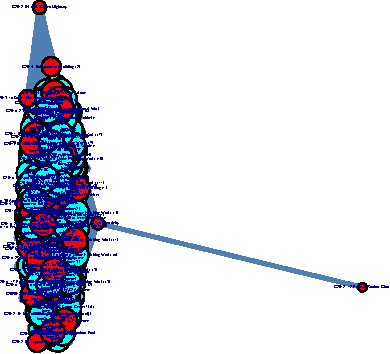
\includegraphics{NDA_DISTS-2} }

}

\caption{Clustered Euclidean distance graph of projects for network and project indicators}\label{fig:NDA_DISTS}
\end{figure}

Figure \ref{fig:NDA_DISTS} shows that both clustering methods provide
two-two clusters.

Considering only network indicators the first cluster contains 32.93\%
synthetic and 67.07\% real project networks, whereas the second cluster
contains 50\% synthetic and 50\% real project networks. Considering only
project indicators, the first cluster contains 43.96\% synthetic and
56.04\% real project networks, whereas the second cluster contains 0\%
synthetic and 100\% real project networks.

\section{Discussion}\label{sec:discussion}

According to the research questions, the network-level indicators are
proposed, thus providing new insight into project planning. The existing
time-, resource-related, and structural indicators and the proposed
network-level indicators of real and synthetic project networks are
compared.

The findings indicate that real projects exhibit variations compared
with synthetic projects in terms of time-related, resource-related,
structural, and network-level characteristics. These variations have
consequences for the scheduling and allocation of project tasks and
resources as well as for the overall performance, risk, and quality of
the project.

The time-related indicators in Table \ref{tab:MEANS_TIME} indicate that
real projects are less flexible and efficient than synthetic projects.
This is evident from their longer and more variable durations, longer
and more constrained critical paths, fewer and less flexible noncritical
tasks, and greater slack per activity and per critical path length. The
project manager must be cognizant of these problems and strategically
plan in response.

The resource-related indicators (Table \ref{tab:MEANS_RESOURCE}) confirm
that real projects are also less flexible and efficient than are the
synthetic projects in terms of resource planning and allocation, as they
have more types and higher demands of resources, lower efficiency and
utilization, less resource distribution and diversity, lower resource
feasibility and strength, greater resource inequality and concentration,
less resource tightness and constrainedness, and more resource excess
and underutilization.

The structural and network-level indicators (Table
\ref{tab:MEANS_LOGIC}) demonstrate that real projects exhibit higher
connectedness and reduced complexity compared with those of synthetic
projects in terms of the project network and project schedule. Real
projects that exhibit a greater number of arcs per node indicates a
greater number of connections between activities, a more evenly
distributed allocation of activities, simple and less crowded project
networks, increased flexibility and reduced constraints, more fragmented
and modular networks, heightened vulnerability to targeted disruptions,
a greater presence of triangles and clustering of activities, positive
assortativity, lower modularity, higher centrality, lower efficiency,
and higher transitivity.

The ANOVA results (Table \ref{tab:ANOVA}) reveal the significant factors
in each indicator group, corroborating the descriptive statistics and
emphasizing the primary distinctions between the real and synthetic
projects. These factors can be utilized to classify projects via
supervised and unsupervised learning classification techniques; thus,
enhancing the processes of project selection and prioritizing. According
to Table \ref{tab:ANOVA}, Figure \ref{fig:Boruta} also shows that
network indicators have an important role in describing a project
network. The results confirm that the network structure of real projects
is significantly different than that of synthetic projects.

The results of the employed GNDA method in unsupervised clustering also
confirm that, on the basis of the correlation between indicators,
four-four clusters can be specified for both synthetic and real
projects. Nevertheless, these clusters do not fully follow the grouping
found in the literature. In addition, network indicators can be found in
most clusters, which suggests that network indicators affect all types
of indicators (see Figure \ref{fig:NDA_SYNPROJ}).

If we reverse the clustering and group project networks, we see that we
can obtain two-two each on the basis of the project and the proposed
network-level indicators. On the basis of the project indicators, one
group is purely synthetic, whereas the other group contains a mixture of
real and synthetic projects. However, if only network indicators are
considered, We obtain more mixed clusters. Moreover, the supervised
learning results as in Figure \ref{fig:Boruta}) show that the indicators
together separate the project networks well.

The differences in flexibility and efficiency between real and synthetic
projects could be attributed to the idealized nature of synthetic
datasets, which may not fully capture the complexities and constraints
of real-world project management. Real projects often face unforeseen
challenges, resource limitations, and external dependencies that are not
typically modeled in synthetic datasets. Agile methodologies could
potentially address these differences by promoting adaptability,
continuous reassessment, and iterative planning. The proposed unified
matrix planning (UMP) model can support this agile approach by allowing
flexible project structures and enabling the prioritization of
activities \citep{kosztyan2023matrix}. \citet{kosztyan2023matrix} showed
that the UMP model's ability to store both fixed and flexible project
structures suggests that it could facilitate the dynamic reassessment of
task relationships and priorities, which is crucial in agile project
management. In addition, \citet{kosztyan2023matrix} also noted that by
introducing task priorities, the traditional project indicators of the
resulting flexible project structures are also closer to the idealized
indicators of synthetic projects. However, it is an open question
whether this is also true for the network-level indicators now proposed.
By providing a framework that can represent and analyze both ideal
(synthetic) and real project networks, the UMP model could help
practitioners identify areas where real projects deviate from ideal
conditions and guide them in implementing more flexible and efficient
project management practices.

Traditional project indicators and the proposed network-level indicators
offer complementary perspectives on project analysis, with some
alignments and contrasts. Traditional indicators focus on time,
resources, and structural aspects, whereas network-level indicators
provide insights into the project's network properties. Both types of
indicators measure complexity, but in different ways. For instance, the
traditional `coefficient of network complexity' (CNC) measures
connectedness, whereas network-level indicators such as `density' and
`average path length' offer more nuanced views of network structure.
Time-related indicators like `slack' have some correlation with the
network centrality measures, as tasks with high centrality often have
less slack. Resource-related indicators do not have direct counterparts
in network-level indicators, but network measures can indirectly reflect
resource distribution. Structural indicators such as `order strength'
(OS) align somewhat with network modularity measures, both reflecting
the project's organizational structure. However, network-level
indicators provide additional insights into project robustness,
efficiency, and hierarchical structure that is not captured by
traditional indicators.

\section{Summary and conclusion}\label{sec:conclusion}

In this study, we introduced and examined network-level indicators for
activity-on-node project networks, in addition to the preexisting
time-related, resource-related, and structural indicators. The
network-level indicators are derived from the principles of network
theory and graph analysis. These indicators offer fresh perspectives on
the qualities and attributes of the project network, including density,
diameter, modularity, centrality, resilience, efficiency, and
transitivity. Moreover, such indicators can measure emergent and
nonlinear characteristics of the project network, including the level of
uniformity, integration, hierarchy, and coherence of the network
structure. These aspects are not measured by the logic indicators, which
are derived from project management theory and logical analysis. These
indicators have the ability to uncover concealed and unforeseen patterns
and behaviors within the project network, which can have an impact on
project performance, risk, and quality (see Contribution \nameref{C1}).

A comparison between synthetic and real project networks, was conducted
by focusing on project and network-level indicators, and we found the
primary distinctions and similarities between them. In this study, we
identified several distinct characteristics that differentiate real
projects from synthetic projects. These include flexibility, efficiency,
diversity, complexity, connectedness, modularity, centrality, resilience
and efficiency. These variations affect scheduling and the allocating of
resources in a project, as well as for project management and
evaluation. In this paper, we propose utilizing supervised and
unsupervised learning classification methods for classification projects
according to their indicator values. This can enhance the processes of
project selection and prioritizing (see Contribution \nameref{C3}).

We have made significant contributions to the current body of
literature. in multiple ways. We presented a novel approach to project
networks analysis, which uses network theory and graph analysis. This
approach can enhance and expand the current understanding, which is
mostly on the basis of project management theory and logical analysis
(\nameref{C1}). Furthermore, we investigated the correlations at the
network level. indicators and the current project indicators, uncovering
the impact of network features on project aspects and the reciprocal
influence they have on each other (\nameref{C2}). This analysis
highlights the potential for integrating and aligning these factors to
enhance project management. Furthermore, we assessed the soundness and
the relevance of the simulation model. We found disparities between real
and synthetic project networks, thereby facilitating enhancements to the
simulation model and project network analysis (\nameref{C3}).

The study has also yielded practical ramifications for scholars and
managers. We showed that network theory and graph analysis are valuable
and applicable for project network analysis (\nameref{C1}). A thorough
and organized framework has also been presented for evaluating and for
comparing project- and network-level indicators (\nameref{C2}). We
provided managers with fresh perspectives and resources to comprehend,
to oversee, and to enhance the structure and performance of the project
network, as well as to handle uncertainties, alterations and
interruptions. We also proposed methods for choosing and ranking
projects on the basis of their indicator values, which can enhance the
efficiency of resource allocation and strategy implementation
(\nameref{C3}).

\section{Limitations and future directions}\label{sec:limitations}

This study has limitations that could be addressed in future work. The
study focuses primarily on static project networks, whereas real
projects often have dynamic structures that change over time. Developing
methods to analyze and compare dynamic project networks could be
valuable extension of this work. Additionally, the study does not
consider the impact of external factors such as risk and uncertainty on
project networks. Incorporating these elements into the analysis could
provide more robust insights for project management.

Limitations of the proposed network properties in complex project
networks, several areas warrant further investigation. The density
measure, for instance, may not adequately captures the nuances of highly
interconnected project networks, where the quality of connections might
be more important than their quantity. Modularity measures could be
refined to better reflect the practical groupings of tasks in real
projects, which may not always align with purely structural divisions.
Other network-level indicators, such as centrality measures, might need
to be adapted to account for the unique characteristics of project
networks, such as temporal dependencies and resource constraints. Future
research could explore how these network properties can be modified or
complemented to provide more meaningful insights in the context of
complex project management. Additionally, developing new indicators that
specifically address the challenges of large-scale, multimodal projects
could significantly enhance our understanding complex project networks.

\section*{Declarations}

\subsection*{Ethics approval and consent to participate}

Not applicable.

\subsection*{Consent for publication}

Not applicable.

\subsection*{Availability of data and materials}

Data and functions are freely available and it can be downloaded from
the CRAN websites. The applied packages and data are listed in the
Section \ref{sec:background}. Both the entire article and all analysis
is implemented by R in RStudio.

\subsection*{Competing interests}

The author retains full responsibility for the content of this
publication and there are no competing interests.

\subsection*{Funding}
\label{s:acknowledgements}

This work was performed for the TKP2021-NVA-10 project with support
provided by the Ministry of Culture and Innovation of Hungary from the
National Research, Development and Innovation Fund, financed under the
2021 Thematic Excellence Programme funding scheme. Zsolt T. Kosztyán's
research contribution supported by Project no. K 142395 was implemented
with support provided by the Ministry of Culture and Innovation of
Hungary from the National Research, Development and Innovation Fund,
financed under the K\_22 ``OTKA'\,' funding scheme.

\subsection*{Authors' contributions}

Not applicable.

\subsection*{Acknowledgments}

We would like to thank the University of Pannonia for supporting
Dr.~Zsolt T. Kosztyán. We would also like to thank the Hungarian
Ministry of Culture and Innovation for funding Dr.~Zsolt T. Kosztyán.

\bibliography{bibliography.bib}

\renewcommand\bibliography[1][]{}

\clearpage
\pagenumbering{arabic}
\renewcommand{\thepage}{A-\arabic{page}}

\begin{appendices}

\section{Formal description of applied indicators}\label{sec:app_net}

An activity-on-node project network is a set of nodes
(i.e.,\textasciitilde tasks) and a set of directed edges
(i.e.,\textasciitilde dependencies) that connect some pairs of tasks. In
matrix-based project planning, both the logic plan and the time and the
resource demands are in a submatrix.

We proposed project indicators, such as time-related, resource-related
and structural (logic) and network-level indicators to describe the
project plan.

\textbf{The applied time-related indicators are described below.}

Table \ref{tab:DESCTIMERELIND} summarizes the applied time-related
indicators. A detailed formal description is provided in the
Supplementary material.

\begingroup\fontsize{8}{10}\selectfont

\begin{longtable}[t]{l>{\raggedright\arraybackslash}p{2.4cm}>{\raggedright\arraybackslash}p{2.7cm}>{\raggedright\arraybackslash}p{4.3cm}}
\caption{\label{tab:DESCTIMERELIND}Description of time-related indicators}\\
\toprule
\textbf{ID} & \textbf{Variable name} & \textbf{Short description (what it measures)} & \textbf{Why is it important to measure in an activity-on-node project network?}\\
\midrule
\endfirsthead
\caption[]{Description of time-related indicators \textit{(continued)}}\\
\toprule
\textbf{ID} & \textbf{Variable name} & \textbf{Short description (what it measures)} & \textbf{Why is it important to measure in an activity-on-node project network?}\\
\midrule
\endhead

\endfoot
\bottomrule
\endlastfoot
XDUR & average activity duration & Sum of activity durations divided by the number of activities. & Shows the average units of the durations in projects.\\
\cmidrule{1-4}\pagebreak[0]
VADUR & variance in activity durations & Variance in the duration of activities. & Likely to have an effect on scheduling on the basis of activity duration.\\
\cmidrule{1-4}\pagebreak[0]
MAXCPL & maximum critical path length & Total project time or the longest critical path length. & The minimal duration of the project / portfolio considering the earliest (resource-unconstrained) start schedule.\\
\cmidrule{1-4}\pagebreak[0]
NSLACK & number of activities with positive (nonzero) total float & Counts total number of nonzero activity float(s) & \\
\cmidrule{1-3}\nopagebreak
PCTSLACK & percentage of activities with positive (nonzero) total float & The ratio of nonzero activity float(s) and all activities. & \\
\cmidrule{1-3}\nopagebreak
TOTSLACK\_R & total slack ratio & Total slack (float) of all activities divided by the critical path length. & \\
\cmidrule{1-3}\nopagebreak
XSLACK & average slack & Average total slack per activity & \\
\cmidrule{1-3}\nopagebreak
XSLACK\_R & average slack ratio & Average slack ratio on the critical path & \multirow{-5}{4.3cm}{\raggedright\arraybackslash Reflects scheduling freedom in the sense that specific activities can be delayed without delaying the completion of a project.}\\
\cmidrule{1-4}\pagebreak[0]
NFREESLK & number of activities with positive (nonzero) free slack & Counts total number of nonzero activity slack(s) & \\
\cmidrule{1-3}\nopagebreak
PCTFREESLK & percentage of activities with positive (nonzero) free slack & The ratio of nonzero activity slack(s) and all activities & \\
\cmidrule{1-3}\nopagebreak
XFREESLK & average free slack & Average free slack per activity & \multirow{-3}{4.3cm}{\raggedright\arraybackslash Reflects scheduling freedom of specific activities can be delayed without delaying any other starts of the activities in the project.}\\*
\end{longtable}
\endgroup{}

\begin{itemize}
\item
  \textbf{Average activity duration} (XDUR): This indicator reflects the
  average amount of time it takes to complete an activity in a project.
  It is important to measure the XDUR because it helps to estimate the
  total duration of the project, even if the given scheduling algorithms
  initiate activities later. The average task duration is calculated as
  \begin{equation}
  \label{eq:XDUR}
  \text{XDUR}:=\frac{1}{n}\sum_{i=1}^n d_{i}
  \end{equation} \noindent where \(n\) is the number of tasks and
  \(d_i\) is the duration of the \(i\)-th task.
\item
  \textbf{Variance in activity duration} (VADUR): This indicator
  measures the variability or dispersion of the activity durations in a
  project. It is important to measure VADUR because it helps to assess
  the uncertainty and the risk of the project schedule, which is
  necessary to plan for contingencies and buffers. The variance in task
  duration is calculated as follows: \begin{equation} 
  \label{eq:VADUR} 
  \text{VADUR}:=\frac{1}{n-1}
  \sum_{i=1}^{n}\left( d_{i}-\overline{X}\textnormal{DUR}\right) ^{2}
  \end{equation}
\item
  \textbf{Maximum critical path length} (MAXCPL): This indicator is
  expressed as the total project time or the longest sequence of
  activities from the start node to the end node in an AoN project
  network. It is important for measuring the MAXCPL because it
  determines the minimum time required to complete the project, and any
  delay in an activity on the critical path delays the whole project. We
  can denote MAXCPL as a \emph{total project time} (TPT)
\item
  \textbf{Number of activities with positive (nonzero) total float}
  (NSLACK): This indicator counts the total number of activities that
  have some slack or float in a project. Slack or float is the amount of
  time an activity can be delayed without affecting the project
  completion date. It is important to measure NSLACK because it
  indicates the degree of flexibility or buffer in the project schedule,
  as well as potential opportunities for resource leveling or smoothing.
  Formally: \begin{equation}
  \label{eq:NSLACK}
  \text{NSLACK}=\sum_{i=1,TS_i>0}^n l_{ii}
  \end{equation} \noindent where \(LS_i\) (\(ES_i\)) is the latest
  (earliest) start time, and \(TS_i:=LS_i-ES_i\) is the total slack of
  task \(i\); \(l_{ii}=[\mathbf{LD}]\) is the diagonal value of the
  logic domain.
\item
  \textbf{Percent of activities with positive (nonzero) total float}
  PCTSLACK: This indicator represents the ratio of activities that have
  some slack or float to the total number of activities in a project. It
  is important for measuring PCTSLACK because it reflects the proportion
  of flexibility or buffer in the project schedule and the potential
  opportunities for resource leveling or smoothing. The percentage of
  tasks with positive total slack are calculated as follows:
  \begin{equation}
  \text{PCTSLACK}:=\frac{1}{n} \sum\limits_{i=1}^n\begin{cases} 1 & \text{if $TS_i=LS_i-ES_i > 0$} \\ 
  0 & \text{if $TS_i=LS_i-ES_i = 0$}\end{cases}
  \end{equation}
\item
  \textbf{Total Slack Ratio} (TOTSLACK\_R): This indicator shows the
  ratio of the total slack or float of all activities to the critical
  path length in a project. It is important to measure TOTSLACK\_R
  because it reflects the overall flexibility or buffer in the project
  schedule and the potential opportunities for resource leveling or
  smoothing. The total slack ratio is calculated as follows:
  \begin{equation}
  \label{eq:TOTSLACK_R}
  \text{TOTSLACK\_R}:=\frac{\sum\limits_{i=1}^n TS_i}{TPT}
  \end{equation}
\item
  \textbf{Average slack} (XSLACK): This indicator shows the average
  amount of slack or float per activity in a project. It is important to
  measure XSLACK because it reflects the average flexibility or buffer
  per activity in the project schedule and the potential opportunities
  for resource leveling or smoothing. The average total slack per task
  is calculated as follows: \begin{equation}
  \label{eq:XSLACK}
  \text{XSLACK}:=\frac{1}{n} \sum\limits_{i=1}^n TS_i
  \end{equation}
\item
  \textbf{Average slack ratio} (XSLACK\_R): This indicator shows the
  average ratio of slack or float per activity to the critical path
  length in a project. It is important to measure XSLACK\_R because it
  reflects the average flexibility or buffer per activity in relation to
  project duration and the potential opportunities for resources
  leveling or smoothing. The average slack ratio is calculated as
  \begin{equation}
  \label{eq:XSLACK_R}
  \text{XSLACK\_R}:=\frac{XSLACK}{TPT}
  \end{equation}
\item
  \textbf{Number of activities with positive (nonzero) free slack}
  (NFREESLK): This indicator counts the total number of activities that
  have some free slack in a project. Free slack is the amount of time an
  activity can be delayed without affecting the start of any other
  activity in the project. It is important to measure NFREESLK because
  indicates the degree of flexibility or buffer for specific activities
  in the project schedule and the potential opportunities for resource
  optimization or reallocation. \begin{equation}
  \label{eq:NFREESLACK}
  \text{NSLACK}=\sum_{i=1,FS_i>0}^n l_{ii}
  \end{equation} \noindent where the earliest finishing time of the task
  \(j\) is \(EF_j=ES_j+d_j\); and
  \quad \(FS_i:=\min\limits_{l_{ij}=1} ES_j-EF_i\) is the free slack of
  task \(i\) (lowest early start of successors - early finish).
\item
  \textbf{Percent of activities with positive (nonzero) free slack}
  PCTFREESLK: This indicator reflects the ratio of activities that have
  some free slack to the total number of activities in a project. It is
  important for measuring PCTFREESLK because it reflects the proportion
  of flexibility or buffer for specific activities in the project
  schedule and the potential opportunities for resource optimization or
  reallocation. The percentage of activities that have positive
  (nonzero) free slack can be calculated as follows: \begin{equation}
  \label{eq:PCTFREESLK}
  \text{PCTFREESLK}:=\frac{1}{n} \sum\limits_{i=1}^n\begin{cases} 1 & \text{if $FS_i > 0$} \\ 0 & \text{if $FS_i = 0$}\end{cases}
  \end{equation}
\item
  \textbf{Average free slack} (XFREESLK): This indicator shows the
  average amount of free slack per activity in a project. It is
  important to measure the XFREESLK because it reflects the average
  flexibility or buffer for specific activities in the project schedule
  and the potential opportunities for resource optimization or
  reallocation. \begin{equation}
  \label{eq:XFREESLK}
  \text{XFREESLK}:=\frac{1}{n} \sum\limits_{i=1}^n FS_i
  \end{equation}
\end{itemize}

\textbf{Formal definitions of the employed resource indicators:}

Table \ref{tab:DESCRESRELIND} summarizes the applied resource-related
indicators. A detailed formal description is provided in the
Supplementary material.

\begingroup\fontsize{8}{10}\selectfont

\begin{longtable}[t]{l>{\raggedright\arraybackslash}p{2.2cm}>{\raggedright\arraybackslash}p{4.1cm}>{\raggedright\arraybackslash}p{3.5cm}}
\caption{\label{tab:DESCRESRELIND}Description of resource-related indicators}\\
\toprule
\textbf{ID} & \textbf{Variable name} & \textbf{Short description (what it measures)} & \textbf{Why is it important to measure in an activity-on-node project network?}\\
\midrule
\endfirsthead
\caption[]{Description of resource-related indicators \textit{(continued)}}\\
\toprule
\textbf{ID} & \textbf{Variable name} & \textbf{Short description (what it measures)} & \textbf{Why is it important to measure in an activity-on-node project network?}\\
\midrule
\endhead

\endfoot
\bottomrule
\endlastfoot
\cellcolor{gray!10}{NRES} & \cellcolor{gray!10}{number of renewable resources} & \cellcolor{gray!10}{How many resources are available for scheduling activities.} & \cellcolor{gray!10}{Number of renewable resources in the project.}\\
\cmidrule{1-4}\pagebreak[0]
XDMND & average resource demand & Average quantity of resources demanded if required by an activity. & Shows the average units of the resources in projects.\\
\cmidrule{1-4}\pagebreak[0]
\cellcolor{gray!10}{RU} & \cellcolor{gray!10}{resource use} & \cellcolor{gray!10}{Measures for each activity the number of resource types used.} & \cellcolor{gray!10}{How tasks are using resources types. Is a vector of the number of different resources each activity uses.}\\
\cmidrule{1-4}\pagebreak[0]
XUTIL & average resource utilization & The average utilization of resource types on the longest critical path length. & Assessing resource efficiency and identifying resource bottlenecks.\\
\cmidrule{1-4}\pagebreak[0]
\cellcolor{gray!10}{PCTR} & \cellcolor{gray!10}{percentage of activities requiring positive amount of resource type} & \cellcolor{gray!10}{Percentage of activities that require the given resource type} & \cellcolor{gray!10}{How resources are distributed among activities.}\\
\cmidrule{1-4}\pagebreak[0]
RS & resource strength & Measures the availability of resources (normalized) for the earliest start schedule. & Assessing the resource feasibility and identifying the resource gaps for the earliest start schedule.\\
\cmidrule{1-4}\pagebreak[0]
\cellcolor{gray!10}{A\_RS} & \cellcolor{gray!10}{alpha distribution of resource strength} & \cellcolor{gray!10}{Measures the variation (α-distance) of multiple resource strength indicators.} & \cellcolor{gray!10}{Shows the variation of resource strengths in unconnected (sub)prujects.}\\
\cmidrule{1-4}\pagebreak[0]
NARLF & normalized average resource loading factor & Shows whether the resource demands for all projects with the earliest start schedule occur in the first or second half of the critical path duration of the portfolio. & To know whether resource demand is front- or backloaded in the project (portfolio).\\
\cmidrule{1-4}\pagebreak[0]
\cellcolor{gray!10}{GINI} & \cellcolor{gray!10}{Gini coefficient} & \cellcolor{gray!10}{How the total work content (each activity’s renewable resource demand multiplied by its duration) is distributed among all activities.} & \cellcolor{gray!10}{(In)equality of renewable resource profiles among tasks.}\\
\cmidrule{1-4}\pagebreak[0]
RC & resource constrainedness (for each resource type) & Measures per resource type the average quantity demanded by all activities divided by its availability. & Considers the amount of the resource needed.\\
\cmidrule{1-4}\pagebreak[0]
\cellcolor{gray!10}{XCON} & \cellcolor{gray!10}{average resource constrainedness over time} & \cellcolor{gray!10}{Sum of renewable resource demands (divided by the number of non-zero demands) divided by the availability of the given resource type.} & \cellcolor{gray!10}{Reflects the "tightness" of certain resource types.}\\
\cmidrule{1-4}\pagebreak[0]
RF & resource factor & Average portion of resource types requested per activity. & Density of the resource matrix. Does not account for the amount of the resource needs.\\
\cmidrule{1-4}\pagebreak[0]
\cellcolor{gray!10}{TOTOFACT} & \cellcolor{gray!10}{total obstruction factor} & \cellcolor{gray!10}{Excess resource requirements divided by resource work content (duration multiplied by resource demand), measured for the earliest start schedule.} & \cellcolor{gray!10}{Excessive resource needs.}\\
\cmidrule{1-4}\pagebreak[0]
TOTUFACT & total underutilization factor & Total resources need less than available divided by work content (duration multiplied by resource demand) for the earliest start schedule. & Reflects underutilization (demand below availability) of resources.\\*
\end{longtable}
\endgroup{}

We write \(\mathcal{S}\) as a realized project structure and
\(\mathbf{LD} \in \{0,1\}^{n\times n}, \mathbf{T} \in \mathbb{R}_+^n \text{ and } \mathbf{RD} \in \mathbb{R}_+^{n \times \rho}\)
as a domain of the matrix representation of \(\mathcal{S}\), where \(n\)
is the number of tasks and \(|\mathcal{A}| =\sum_{ij, i\neq j} l_{ij}\)
(\(l_{ij}=[\mathbf{LD}]_{ij}\)). We write \(t_i = [\mathbf{TD}]_{ii}\)
as the duration of task \(i\) and TPT as the duration of the project,
and \(r_{ij}=[\mathbf{RD}]_{ij}\) as the resource demand of task \(i\)
of resource \(j\).

\(\overrightarrow{\mathcal{S}}\) is a project schedule of project
structure \(\mathcal{S}\) if for each realized task
\(a_i\in \mathcal{S}\) the interval \(T_i \subseteq [0,\text{TPT}]\) is
determined when \(a_i\) is addressed (scheduled). To ensure
compatibility with other papers, the redundant notation
\(a_i(T)\in \overrightarrow{\mathcal{S}}\) is used.

We write \(S(a_i(T))\in [0,TPT-t_i]\) as the start and
\(F(a_i(T)) \in [t_i,TPT]\) the completion time of task \(i\). The early
schedule, denoted \(\overrightarrow{\mathcal{S}}_{\min}\), satisfies
\(\forall a_i(T)\in \overrightarrow{\mathcal{S}}_{\min}\)
\(S(a_i(T))=\text{ES}_i\) and \(F(a_i(T))=\text{EF}_i\). We write the
\emph{resource demand} \(j\) of task \(i\) at time \(\tau\) as follows:

\begin{equation}
\label{eq:r_ij}
r_{ij}(\tau):=\begin{cases}r_{ij}\text{ if } a_i(T)\in \overrightarrow{\mathcal{S}}, \tau \in T_i \\
0\text{ otherwise}\end{cases}   
\end{equation}

Furthermore, we denote the total (renewable) resource \emph{demand} as
\(j\) at time \(\tau\) as
\(r_j(\tau)=\sum_ir_{ij}(\tau), \text{ where } \tau \in [0,\text{TPT}]\).

\begin{itemize}
\item
  \textbf{The resource Factor} (RF), is the density of \textbf{RD}, the
  resource matrix from a domain mapping matrix (DMM). The RF gives the
  rate of how often resources are needed from all possible resource
  type-activity pairings. Higher RF values indicate a more complex
  scheduling problem. \begin{equation}
    \label{eq:RF}
    \textnormal{RF}
    :=\frac{1}{n\rho}\sum_{i=1}^{n}\sum_{j=1}^{\rho}\begin{cases} 1 & \textnormal{if } r_{ij}>0 \\ 0 & \textnormal{otherwise}  \end{cases} \quad 
    =\frac{1}{\rho}\sum_{j=1}^{\rho}{\textnormal{PCTR}_{j}}
    \end{equation} \noindent where \(r_{ik}\) denotes the amount of
  resource type \(j\) needed by task \(i\) and \(\textnormal{PCTR}_j\)
  denotes the percentage of activities that require the given resource
  type, which is a columnwise view of the RF as follows:
  \begin{equation}
    \label{eq:PCTR}
    \textnormal{PCTR}_{j}:=\frac{1}{n} \sum_{i:=1}^n \begin{cases} 1 & \textnormal{if } r_{ij}>0 \\0 & \textnormal{otherwise}  \end{cases}
  \end{equation}
\item
  \textbf{Resource Use} (RU), represents the resource use for each
  activity, i.e., the number of resource types used. The RU varies
  between 0 and \textit{r} (the number of resource types). It is a
  rowwise view of RF (\(i=1,...,n\)) as follows: \begin{equation}
     \label{eq:RU}
     \textnormal{RU}_i := \sum_{j=1}^{\rho}  \left\{\begin{matrix} 1  &\textnormal{if } r_{ij}>0  \\  0 & \textnormal{otherwise} \end{matrix}\right.
   \end{equation}
\item
  \(\textnormal{DMND}_j\) is \textbf{the average quantity of resources}
  \(j\) demanded when needed by an activity (\(j=1,...,\rho\)) as
  follows: \begin{equation}
  \label{eq:DMND}
    \textnormal{DMND}_j:=\frac{\sum_{i=1}^n r_{ij}}{\sum_{i=1}^n \begin{cases} 1 & \text{if } r_{ij}>0 \\ 0 & \text{if } r_{ij}=0 \end{cases}}
  \end{equation}
\item
  RC is \textbf{the resource constrainedness} of each resource type and
  is calculated as follows: \begin{equation}
  \label{eq:RC}
    \textnormal{RC}_{j}:=\frac{\textnormal{DMND}_{j}}{\alpha_{j}}
  \end{equation} \noindent where \(\alpha_{j}\) is the
  \emph{availability} of renewable resource type \(j\).
\end{itemize}

The following indicators of \citet{patterson1976project} require early
scheduling (\(\overrightarrow{\mathcal{S}}_{\min}\)) of the activities
regarding the precedence relations but not the resource constraints.

\begin{itemize}
\tightlist
\item
  RS is the \textbf{resource strength} of each renewable resource type
  and is calculated as follows: \begin{equation}
  \label{eq:RS}
    \textnormal{RS}_{j}:=\frac{\alpha_{j}-r_{j}^{\min}}{r_{j}^{\max}-r_{j}^{\min}}
  \end{equation} \noindent  where \(\alpha_{j}\) denotes the total
  availability of renewable resource type \(j\),
  \(r_{j}^{\min}:= \max_{i=1,...,n} (r_{ij})\) is the highest
  \emph{individual} resource demand and \(r_{j}^{\max}\) denotes the
  peak total demand at any moment for resource type \(j\) in the
  precedence, preserving the earliest start schedule. The
  \(RS_i^{(\alpha)}\) can be calculated as follows:
\end{itemize}

\begin{equation}
\label{eq:RS_A}
RS_i^{(\alpha)} = \begin{cases}
\frac{RS_i^\alpha - 1}{\alpha}, & \alpha \neq 0 \\
\log(RS_i), & \alpha = 0
\end{cases}
\end{equation} the \(\alpha\)-distance between the RS distributions of
different subprojects or disconnected components of the project network,
which is a measure of how different two distributions are on the basis
of the alpha power transformation. The \(\alpha\)-distance can be
calculated as: \begin{equation}
\label{eq_D_RS}
D_{\alpha}(RS_A, RS_B) = \sqrt{\frac{1}{n} \sum_{i=1}^n (RS_{A,i}^{(\alpha)} - RS_{B,i}^{(\alpha)})^2}
\end{equation} \noindent where \(RS_A\) and \(RS_B\) are the vectors of
RS indicators for subprojects A and B, respectively, and \(n\) is the
number of activities in each subproject. A\_RS indicator, which is the
average \(\alpha\)-distance between the RS distributions of all possible
pairs of subprojects or disconnected components in the project network.
The A\_RS indicator can be calculated as: \begin{equation}
\text{A\_RS} = \frac{2}{m(m-1)} \sum_{A < B} D_{\alpha}(RS_A, RS_B)
\end{equation} \noindent where \(m\) is the number of subprojects or
disconnected components in the project network, and the summation is
over all possible pairs of subprojects or components.

\begin{itemize}
\item
  \(\textnormal{UTIL}_j\) is the \textbf{utilization} (rate) of
  resources, and it is measured on the basis of the critical path
  length. Higher values indicate more constraints, less room for
  scheduling, and less possibility of changing the task starting times
  without increasing the TPT. \begin{equation}
  \label{eq:UTIL}
    \textnormal{UTIL}_{j}:=\frac{\sum_{i=1}^n r_{ij}t_{i}}{\alpha_{j} \cdot \textnormal{TPT}}
  \end{equation}
\item
  The applied XUTIL is the \textbf{average resource utilization}.
\item
  \(\textnormal{TCON}_j\) is the \textbf{constraint on the (renewable)
  resource type} \(j\) over time. In practice, this is the average
  utilization (\(\textnormal{UTIL}_j\)) considering only those tasks
  that use that particular resource type as follows: \begin{equation}
    \textnormal{TCON}_j:=\frac{\sum_{i=1}^n r_{ij}t_{i}}{\alpha_{j} \cdot \textnormal{TPT} \cdot \sum_{i=1}^n \begin{cases} 1 & \textnormal{if } r_{ij}>0 \\0 & \textnormal{otherwise}  \end{cases}}
  \end{equation}
\item
  \(\textnormal{OFACT}_j\) is the \textbf{obstruction factor of
  (renewable) resource type} \(j\) and is calculated as follows:
  \begin{equation}
    \label{eq:OFACT}
     \textnormal{OFACT}_j:=\frac{\int_{0}^\textnormal{TPT}  \max \{0;r_j(\tau)-\alpha_j \} d\tau}{\sum_{i=1}^n r_{ij}t_{i}}
   \end{equation}
\item
  \textbf{Total obstruction factor} (TOTOFACT=\(\sum_jOFACT_j\) is the
  sum of UFACT for resources.
\item
  \(\textnormal{UFACT}_j\) is the \textbf{underutilization factor} and
  is calculated as follows: \begin{equation}
     \textnormal{UFACT}_j:=\frac{\int_{0}^\textnormal{TPT}  \max \{0;\alpha_j - r_j (\tau)\} d\tau}{\sum_{i=1}^n r_{ij}t_{i}}
  \end{equation}
\item
  The \textbf{total underutilization factor}
  (TOTUFACT=\(\sum_jOFACT_j\))): sum of UFACT for resources.
\item
  The \textbf{average resource loading factor} (ARLF), suggested by
  \citet{kurtulus1982multi}, represents the resource distribution of
  projects. If resource requirements are in the first half of the
  project, it has a negative value, whereas a positive value means that
  the resource demands are in the latter half of the project; these
  values are on the basis of the critical path duration of each project.
  For multiple (sub)projects, the possible issue of averaging individual
  ARLF values are managed by NARLF, where normalization is performed
  with the critical path duration of all (sub)projects
  \citep{browning2010resource}. The formula is further improved by
  \citep{van2020resource} with NARLF, which, on top of this, determines
  if a resource demand falls at the beginning or the end on the basis of
  the critical path of the portfolio instead of the critical path for
  each project. It uses two auxiliary variables: \begin{equation}
  \label{eq:ARLF}
  Y_{i(\tau)}=
  \begin{cases}
  1 & \text{if activity } a_{i} \text{ is active at time } \tau,\\
  0 & \text{otherwise}
  \end{cases}
  \end{equation}
\end{itemize}

\begin{equation}
\label{eq:NARLF1}
Z_{i(\tau)}=
\begin{cases}
-1 & \text{if } \tau \leq \lceil TPT/2 \rceil,\\
1 & \text{if } \tau > \lceil TPT/2 \rceil,
\end{cases}
\end{equation}

to obtain:

\begin{equation}
\label{eq:NARLF}
\begin{split}
\text{NARLF} = \frac{1}{TPT} \sum_{\tau}^{TPT} \sum_{i=1}^{n} \sum_{j=1}^{\rho} Z_{i(\tau)} Y_{i(\tau)} \left( \frac{r_{ij}}{|\{r_{ij}:r_{ij}>0\}|}\right)
\end{split}
\end{equation} \noindent  where \(\tau\) is the time for the earliest
start schedule considering release dates.

\begin{itemize}
\tightlist
\item
  The \textbf{Gini coefficient} is a measure of inequality that compares
  the actual distribution of a variable, such as income, wealth, or work
  content, with a hypothetical equal distribution. The Gini coefficient
  formula is: \begin{equation}
  \text{GINI} = \frac{\sum_{i=1}^n \sum_{j=1}^n |x_i - x_j|}{2n^2 \bar{x}}
  \end{equation} \noindent where \(n\) is the number of observations,
  \(x_i\) is the value of the variable for the \(i\)-th observation, and
  \(\bar{x}\) is the mean value of the variable.
\end{itemize}

To apply this formula to the work content of activities, we define the
variable \(x_i\) as the product of the renewable resource and the
duration of the \(i\)-th activity.

The Gini coefficient ranges from 0 to 1, where 0 means perfect equality
(all activities have the same work content) and 1 means perfect
inequality (one activity has all the work content). A higher Gini
coefficient indicates a more uneven distribution of work content among
the activities.

\noindent \textbf{Formal definitions of the employed logic indicators:}

Table \ref{tab:DESCLOGRELIND} summarizes the applied resource-related
indicators. A detailed formal description is provided in the
Supplementary material.

\begingroup\fontsize{8}{10}\selectfont

\begin{longtable}[t]{l>{\raggedright\arraybackslash}p{2.2cm}>{\raggedright\arraybackslash}p{3.6cm}>{\raggedright\arraybackslash}p{3.6cm}}
\caption{\label{tab:DESCLOGRELIND}Description of logic indicators}\\
\toprule
\textbf{ID} & \textbf{Variable name} & \textbf{Short description (what it measures)} & \textbf{Why is it important to measure in an activity-on-node project network?}\\
\midrule
\endfirsthead
\caption[]{Description of logic indicators \textit{(continued)}}\\
\toprule
\textbf{ID} & \textbf{Variable name} & \textbf{Short description (what it measures)} & \textbf{Why is it important to measure in an activity-on-node project network?}\\
\midrule
\endhead

\endfoot
\bottomrule
\endlastfoot
\cellcolor{gray!10}{TASKS} & \cellcolor{gray!10}{number of activities} & \cellcolor{gray!10}{Measures the size of the network as the number of activities.} & \cellcolor{gray!10}{How many activities are present in the project (portfolio).}\\
\cmidrule{1-4}\pagebreak[0]
I2 & serial-parallel (SP) & Measures the closeness to series or parallel graph. & Determines the number of serial activities in the network on the longest chain.\\
\cmidrule{1-4}\pagebreak[0]
\cellcolor{gray!10}{I3} & \cellcolor{gray!10}{activity distribution (AD)} & \cellcolor{gray!10}{Measures the distribution of the activities over the progressive levels on the basis of the width of each progressive level in the network.} & \cellcolor{gray!10}{Measures how the project activities that do not belong to the longest chain are distributed in the network.}\\
\cmidrule{1-4}\pagebreak[0]
I4 & the length of long arcs (LA) & Measures the presence of long precedence relations. The length of an arc is the difference between the progressive level of the end node and the start node. & A lower value indicates many dependencies between two levels of activities; a higher value indicates the presence of many immediate successors at the next level of the network.\\
\cmidrule{1-4}\pagebreak[0]
\cellcolor{gray!10}{I5} & \cellcolor{gray!10}{short arcs (SA)} & \cellcolor{gray!10}{Measures the presence of short precedence relations. The length of an arc is the difference between the progressive level of the end node and the start node.} & \cellcolor{gray!10}{Alternative for I4 (length of long arcs).}\\
\cmidrule{1-4}\pagebreak[0]
I6 & topological float (TF) & Ont the basis of the difference between the progressive and regressive levels of each activity, the topological float indicator is defined as the fractional total topological float in relation to its maximum. & The topological float of a precedence relation is the number of levels that each activity can shift without violating the maximal level of the network.\\
\cmidrule{1-4}\pagebreak[0]
\cellcolor{gray!10}{C} & \cellcolor{gray!10}{network complexity} & \cellcolor{gray!10}{The average number of non-redundant arcs per node.} & \cellcolor{gray!10}{The number of redundant arcs should not have an influence on project complexity.}\\
\cmidrule{1-4}\pagebreak[0]
CNC & coefficient of network complexity & A measure of the connectedness of a graph takes redundant nodes into account. & A higher complexity means greater connectedness of the network. However, many network problems become easier with increasing CNC.\\
\cmidrule{1-4}\pagebreak[0]
\cellcolor{gray!10}{OS} & \cellcolor{gray!10}{order strength} & \cellcolor{gray!10}{The number of precedence relations (including the transitive ones) divided by the theoretical maximum number of precedence relations.} & \cellcolor{gray!10}{Assessing the complexity and flexibility of the project network and the project schedule.}\\
\cmidrule{1-4}\pagebreak[0]
TDENSITY & total activity density & Measure the interconnectedness of a network. The sum of the maximal number of predecessors minus successors of each activity. & Influences when (in terms of network logic) an activity can be scheduled\\
\cmidrule{1-4}\pagebreak[0]
\cellcolor{gray!10}{XDENSITY} & \cellcolor{gray!10}{average activity density} & \cellcolor{gray!10}{Sum of the maximal number of predecessors minus successors of each activity, divided by the number of activities} & \cellcolor{gray!10}{Influences when (in terms of network logic) an activity can be scheduled}\\
\cmidrule{1-4}\pagebreak[0]
AP & number of articulation points & The number of tasks (and their dependencies) to remove to disconnect the graph (cut vertices). & Removing of articulation points increases the number of connected components in a graph.\\
\cmidrule{1-4}\pagebreak[0]
\cellcolor{gray!10}{COMPS} & \cellcolor{gray!10}{components} & \cellcolor{gray!10}{Size of the largest (strongly) connected component.} & \cellcolor{gray!10}{The robustness of the network against disruptions.}\\
\cmidrule{1-4}\pagebreak[0]
MEAN\_DEGREE & degrees & The average number of dependencies connected to each task. & The average degree of each task.\\
\cmidrule{1-4}\pagebreak[0]
\cellcolor{gray!10}{NARC} & \cellcolor{gray!10}{number of arcs} & \cellcolor{gray!10}{Number of arcs (precedence relationships).} & \cellcolor{gray!10}{How many dependencies each task have.}\\*
\end{longtable}
\endgroup{}

We denote \(\mathcal{S}\) as a realized project structure,
\(\mathbf{LD} \in \{0,1\}^{n\times n}\) of \(\mathcal{S}\);
\(|\mathcal{A}| = \sum_{i \neq j} l_{ij}\)
(\(l_{ij}=[\mathbf{LD}]_{ij}\)) is the total number of dependencies
(arcs) between tasks.

\begin{itemize}
\item
  TASKS=\(I_1\), the \textbf{number of tasks} (nodes), is calculated as
  follows: \begin{equation}
  \label{eq:I1}
    I_1:=n
  \end{equation}
\item
  \(I_2\), the serial-parallel structure, measures the closeness to
  serial or parallel completion. For \(I_2\), the following notation is
  used: \(S_i\) (\(P_i\)) denotes the \emph{set} of immediate successors
  (predecessors) of task \(i\). For topologically ordered, acyclic
  project networks, \(|S_i|=\sum\limits_{j=i+1}^n l_{ij}\),
  \(|P_i|=\sum\limits_{j=1}^{i-1} l_{ji}\). The progressive (\(PL_i\))
  and the regressive (\(RL_i\)) level \emph{numbers} of each task \(i\)
  can be calculated as follows: \begin{equation}
   \label{eq:PLi}
   PL_i := \begin{cases} 
  1 & \text{if $P_i = \emptyset $} \\
  \max\limits_{j \in P_i} PL_j + 1 
  & \text{if $P_i \neq \emptyset $} 
  \end{cases} 
  \end{equation}
\end{itemize}

\noindent  and

\begin{equation}
\label{eq:RLi}
RL_i := \begin{cases} m & \text{ if }S_i = \emptyset \\
\min\limits_{j \in S_i} RL_j - 1 & \text{ if } S_i \neq 
\emptyset 
\end{cases}
\end{equation} \noindent  where \(m=\max\limits_{i} PL_i\). Next, we
have the following: \begin{equation}
\label{eq:I2}
    I_2:=\begin{cases} 1 & \text{if $n = 1$} \\ \frac{m-1}{n-1} & \text{if $n > 1$}\end{cases}
\end{equation}

\begin{itemize}
\tightlist
\item
  \(I_3\), the task distribution, measures the distribution of tasks
  over the progressive levels by calculating the total absolute
  deviations.
\end{itemize}

First, we define the \(j\)-th progressive \emph{level} of \(j=1,...,m\)
as follows: \(\mathbf{PL}_{j}:=\left\{i\leq n:PL_{i}=j\right\}\), i.e.,
the \emph{set} of all tasks having progressive level number \(j\). Then,
\begin{equation}
\label{eq:I3}
    I_3:=\begin{cases} 0 & \text{if $m=1$ or $m =n$} \\ \frac{\alpha_w}{\alpha_{\max}}= \frac{
\sum\limits_{j=1}^m |w_{j} - \overline{w}| }{2(m-1)(\overline{w}-1)} & \text{if $1<m<n$}\end{cases}
\end{equation} \noindent  where \(w_{j}=|\mathbf{PL}_{j}|\) is the width
(size) of progressive level \(j=1,...,m\), \(w=(w_1,w_2,...,w_m\) is the
vector which contains the widths of each progressive level, and
\(\overline{w}=n/m\), \(\alpha_{w}\) is the total absolute deviation
from the average width. Then, \(\alpha_{\max}\) is the maximal value of
\(\alpha_{w}\) of a network (ranging for all possible \(\mathcal{A}\));
thus,
\footnote{The maximal value of $\alpha _{w}$ is achieved ($n$ and $m$ are fixed, $\sum_{j=1}^{m}w_{j}=n$) when all levels are singletons, except for one with $n-\left( m-1\right)$ tasks; repetitive use of the inequality $\left\vert a-\overline{w}\right\vert +\left\vert b-\overline{w}\right\vert <\left\vert a-1-\overline{w}\right\vert +\left\vert b+1-\overline{w}\right\vert$ for $1<a\leq \overline{w}\leq b<n$ produces this extrema. 
} \quad \(\alpha_{\max}=(m-1)(\overline{w}-1)+(n-m+1-\overline{w})\)
\quad this formula simplifies to \(\alpha_{\max}\)
\(=2(m-1)(\overline{w}-1)\). \medskip

\begin{itemize}
\item
  \(I_4\), the ratio of \textit{short} arcs. The length of an ``arc'\,'
  (called a path in graph theory) between tasks \(i_1\) and \(i_2\) is
  defined as \% \quad \$L ( i\_1 , i\_2 ) := \textbar{} PL\_\{i\_1\} -
  PL\_\{i\_2\} \textbar{} \$, \% \quad i.e., the difference between
  their progressive level numbers. Arcs of length \(1\) are called
  \textit{short}, and \%
  \quad \(D:=\sum\limits_{j=1}^{m-1}{w_j}\cdot{w_{j+1}}\) is the
  \textit{maximal} number of short arcs. \(n'_L\) denotes the number of
  arcs of length \(L\) for \(1\leq L \leq m-1\). Then, \(I_4\) is
  calculated as follows: \begin{equation}
  \label{eq:I4}
    I_4:=\begin{cases} 1 & \text{if $D = n - w_1$} \\ \frac{n'_1-n+w_1}{D-n+w_1} & \text{if $D > n - w_1$}\end{cases}
  \end{equation}
\item
  \(I_5\), the ratio of \emph{long} arcs (\(L>1\)), is calculated as
  follows: \begin{equation}
  \label{eq:I5}
    I_5:=\begin{cases} 1 & \text{if $| \mathcal{A} | = n - w_1$} \\ \frac{\left(\sum\limits_{L=2}^{m-1}n'_L\frac{m-L-1}{m-2}\right)+n'_1-n+w_1}{| \mathcal{A} |-n+w_1} & \text{if $| \mathcal{A} |  > n - w_1$}\end{cases}
  \end{equation}
\item
  \(I_6\), the topological float, considers the differences between the
  regressive and the progressive level numbers of task \(i\), i.e.,
  \(|RL_i -PL_i|\), as follows: \begin{equation}
  \label{eq:I6}
    I_6:=\begin{cases} 0 & \text{if $m \in{\{1,n\}}$} \\ \frac{\sum\limits_{i=1}^{n} | RL_i-PL_i |} {(m-1)(n-m)}& \text{if $m \notin{\{1,n\}}$}\end{cases}
  \end{equation}
\item
  CNC, the \textbf{coefficient of network complexity}, is calculated as
  follows: \begin{equation}
  \label{eq:cnc}
  \text{CNC}=\frac{|\mathcal{A}|}{n}
  \end{equation}
\item
  OS, the \textbf{order strength}, is calculated as follows:
  \begin{equation}
  \label{eq:OS}
  \text{OS}=\frac{|\mathcal{A}|}{n(n-1)/2}
  \end{equation}
\item
  C, the \textbf{network complexity}, is calculated as follows:
  \begin{equation}
  \label{eq:C}
  \text{C}=\begin{cases} \frac{\log\frac{|\mathcal{A}|}{n-1}}{\log\frac{n^2-1}{4(n-1)}} & \text{if $n$ is odd} \\   \frac{\log\frac{|\mathcal{A}|}{n-1}}{\log\frac{n^2}{4(n-1)}} & \text{if $n$ is even}\end{cases}
  \end{equation}
\item
  TDENSITY, the \textbf{total activity density}, is calculated as
  follows: \begin{equation}
  \label{eq:TDENSITY}
  \text{TDENSITY}:=
  %\sum_{i:=1}^n\max\left\{0, \sum_{j:=1}^nl_{ji}-\sum_{j:=1}^nl_{ij}\right\}, i\neq j
  \sum_{i:=1}^n\max \left\{0, |P_i|-|S_i| \right\}
  \end{equation}
\end{itemize}

\noindent  \(S_i\) and \(P_i\) were defined immediately before \(I_2\).

\begin{itemize}
\tightlist
\item
  XDENSITY, the \textbf{average activity density}, is calculated as
  follows: \begin{equation}
  \text{XDENSITY}:=\frac{\text{TDENSITY}}{n}\label{eq:XDENSITY} 
  \end{equation}
\end{itemize}

\textbf{Formal definitions of the employed network-level indicators:}

Table \ref{tab:DESCNETRELIND} summarizes the applied resource-related
indicators. A detailed formal description is provided in the
Supplementary materials.

\begingroup\fontsize{8}{10}\selectfont

\begin{longtable}[t]{l>{\raggedright\arraybackslash}p{2.2cm}>{\raggedright\arraybackslash}p{3.8cm}>{\raggedright\arraybackslash}p{4.2cm}}
\caption{\label{tab:DESCNETRELIND}Description of logic indicators}\\
\toprule
\textbf{ID} & \textbf{Variable name} & \textbf{Short description (what it measures)} & \textbf{Why is it important to measure in an activity-on-node project network?}\\
\midrule
\endfirsthead
\caption[]{Description of logic indicators \textit{(continued)}}\\
\toprule
\textbf{ID} & \textbf{Variable name} & \textbf{Short description (what it measures)} & \textbf{Why is it important to measure in an activity-on-node project network?}\\
\midrule
\endhead

\endfoot
\bottomrule
\endlastfoot
\cellcolor{gray!10}{Dens} & \cellcolor{gray!10}{density} & \cellcolor{gray!10}{How many dependencies exist in the project network} & \cellcolor{gray!10}{Degree of complexity of the project network}\\
Diam & diameter & The longest shortest distance between any pair of tasks in the project network. & The degree of dispersion or concentration of the project network.\\
\cellcolor{gray!10}{AVPL} & \cellcolor{gray!10}{average path length} & \cellcolor{gray!10}{Average shortest distance between any pair of tasks in the project network} & \cellcolor{gray!10}{The degree of dispersion or concentration of the project network.}\\
VAs & vertex asymmetries & How asymmetric the network is in terms of the distribution of dependencies among the tasks. & The degree of inequality or diversity in the network structure.\\
\cellcolor{gray!10}{Mot} & \cellcolor{gray!10}{number of motifs} & \cellcolor{gray!10}{The number of recurring patterns of dependencies in the project network.} & \cellcolor{gray!10}{The degree of regularity or randomness of the network.}\\
\addlinespace
ASSORT & assortativity & How similar the nodes are in terms of their degree; the degree is the number of connections they have. & Revealing the degree of homogeneity or heterogeneity in the project network structure\\
\cellcolor{gray!10}{LeM} & \cellcolor{gray!10}{Leiden's graph modularity value} & \cellcolor{gray!10}{How well the network can be partitioned into communities.} & \cellcolor{gray!10}{Degree of diversity or cohesion in the project network.}\\
IM & Infomap's graph modularity value & How well the network can be partitioned into communities. & Degree of diversity or cohesion in the project network.\\
\cellcolor{gray!10}{SGM} & \cellcolor{gray!10}{Spin-Glass graph modularity value} & \cellcolor{gray!10}{How well the network can be partitioned into communities.} & \cellcolor{gray!10}{Degree of diversity or cohesion in the project network.}\\
DZI & in-degree centralization & How concentrated the dependencies are on a few activities & The degree of dependency that some activities have over others.\\
\addlinespace
\cellcolor{gray!10}{DZO} & \cellcolor{gray!10}{out-degree centralization} & \cellcolor{gray!10}{How concentrated the dependencies are on a few activities} & \cellcolor{gray!10}{Degree of influence that some activities have over others.}\\
DZ & degree centralization & How concentrated the dependencies are on a few activities & Degree of dependency and influence that some activities have over others.\\
\cellcolor{gray!10}{CZ} & \cellcolor{gray!10}{closeness centralization} & \cellcolor{gray!10}{How close a task is to all other tasks in the network, on the basis of the sum of the shortest distances between them.} & \cellcolor{gray!10}{Degree of accessibility or reachability that some tasks have in the network.}\\
HZ & harmonic centralization & How close a task is to all other tasks in the network, which is on the basis of the harmonic mean of the distances between them. & The degree of efficiency or effectiveness that some tasks have in the project network.\\
\cellcolor{gray!10}{EZ} & \cellcolor{gray!10}{eigenvector centralization} & \cellcolor{gray!10}{How connected a task is to other well-connected tasks in the network, on the basis of the eigenvector of the adjacency matrix.} & \cellcolor{gray!10}{Degree of importance that some tasks have in the project network}\\
\addlinespace
PRZ & PageRank centralization & How influential or critical a task is for overall project performance. & The degree of impact that some tasks have on the project network.\\
\cellcolor{gray!10}{AZ} & \cellcolor{gray!10}{alpha centralization} & \cellcolor{gray!10}{This measures how centralized the network is as a whole, on the basis of the alpha index.} & \cellcolor{gray!10}{Degree of hierarchy or equality in the project network structure.}\\
PZ & power centralization & This measures how centralized the network is as a whole on the basis of the power index. & Degree of dominance or balance in the project network structure.\\
\cellcolor{gray!10}{BZ} & \cellcolor{gray!10}{betweenness centralization} & \cellcolor{gray!10}{How often a task lies on the shortest path between two other tasks.} & \cellcolor{gray!10}{Degree of intermediation that some tasks have in the project network.}\\
BEZ & edge-betweenness centralization & How often an edge lies on the shortest path between two tasks & The degree of vulnerability or robustness of the project network.\\
\addlinespace
\cellcolor{gray!10}{RRes} & \cellcolor{gray!10}{resilience for random attack} & \cellcolor{gray!10}{How well the network can maintain its connectivity when a fraction of tasks are randomly removed.} & \cellcolor{gray!10}{Degree of robustness or susceptibility of the network.}\\
SRes & resilience for systematic attack & How well the network can maintain connectivity when a fraction of (high-degree) tasks are systematically removed. & Degree of robustness or susceptibility of the network.\\
\cellcolor{gray!10}{ALE} & \cellcolor{gray!10}{average local efficiency} & \cellcolor{gray!10}{Average efficiency of the subgraphs induced by the dependencies of each task in the project network.} & \cellcolor{gray!10}{Degree of redundancy or fragility of the project network.}\\
GE & global efficiency & Average efficiency of the network as a whole. & Degree of redundancy or fragility of the project network.\\
\cellcolor{gray!10}{Tra} & \cellcolor{gray!10}{graph transitivity} & \cellcolor{gray!10}{Ratio of ratio of triangles to triplets in an project network.} & \cellcolor{gray!10}{Degree of cliquishness or openness of the project network.}\\*
\end{longtable}
\endgroup{}

\begin{itemize}
\item
  \textbf{Density} (Dens): This measures how many dependencies exist in
  the project network, relative to the maximum possible number of
  dependencies. A high density means that the project network is more
  connected, whereas a low density means that the network is sparser.
  This indicator reflects the degree of complexity of the project
  network. The density of a network with \(n\) tasks and \(m\)
  dependencies are given by a directed network. \begin{equation}
  Dens = \frac {m} {n(n-1)} \label{eq:Dens}
  \end{equation}
\item
  \textbf{Diameter} (Diam): This measures the longest shortest distance
  between any pair of tasks in the project network (without considering
  task durations). A high diameter means that the network is more
  dispersed, whereas a low diameter means that the network is more
  compact. \emph{This indicator reflects the degree of dispersion or
  concentration of the project network.} The diameter of a network is
  given by \begin{equation}
  Diam = \max_{u,v \in V} d(u,v) \label{eq:Diam}
  \end{equation} \noindent where \(V\) is the set of tasks and
  \(d(u,v)\) is the shortest path distance between tasks \(u\) and \(v\)
\item
  \textbf{Average path length} (AVPL): This measures the average
  shortest distance between any pair of tasks in the project network
  (without considering task durations). A high average path length means
  that the network is more dispersed, while a low average path length
  means that the network is more compact. \emph{This indicator also
  reflects the degree of dispersion or concentration of the project
  network}. The average path length of a network is given by
  \begin{equation}
  AVPL = \frac {1} {n(n-1)} \sum_{u,v \in V} d(u,v) \label{eq:AVPL}
  \end{equation} \noindent
\item
  \textbf{Vertex asymmetries} (VAs): A task with a high vertex asymmetry
  may be a bottleneck, a source of risk in the network, or a task that
  needs more coordination or communication. The average value of the
  vertex asymmetries measure how asymmetric the network is in terms of
  the distribution of dependencies among the tasks. A high vertex
  asymmetry means that the network is more skewed, whereas a low vertex
  asymmetry means that the network is more balanced. \emph{This
  indicator reflects the degree of inequality or diversity in the
  network structure.} The vertex asymmetry of a network is given by
  \begin{equation}
  VAs = \frac {1} {n(n-1)} \sum_{u,v \in V} |k_u - k_v|
  \end{equation} \noindent where \(V\) is the set of tasks and \(k_u\)
  and \(k_v\) are the degrees of tasks \(u\) and \(v\), respectively.
\item
  \textbf{Number of motifs} (Mot): This metric measures the number of
  recurring patterns of dependencies in the project network. A high
  number of motifs means that the project network has a rich structure,
  while a low number of motifs means that the project network has a
  simple structure. \emph{This indicator reflects the degree of
  regularity or randomness of the network.} The number of motifs in a
  network is given by \begin{equation}
  M = \sum_{s \in S} f_s \label{eq:Mot}
  \end{equation} \noindent   where \(S\) is the set of all possible
  subgraphs and \(f_s\) is the frequency of subgraph \(s\) in the
  network.
\item
  \textbf{Assortativity} (Assort): This measures how similar the tasks
  are in terms of their degree, which is the number of dependencies they
  have. A positive assortativity means that tasks tend to depend on or
  influence other tasks that have similar degrees, while a negative
  assortativity means that tasks tend to depend on or influence other
  tasks that have different degrees. \emph{This indicator represents the
  degree of homogeneity or heterogeneity in the project network
  structure.} The assortativity of a network is given by
  \begin{equation}
  r = \frac {\sum {i,j} A{ij}(k_i - \bar{k})(k_j - \bar{k})} {\sum {i,j} A{ij}(k_i - \bar{k})^2}\label{eq:Assort}
  \end{equation} \noindent where \(A_{ij}\) is the adjacency matrix,
  \(k_i\) and \(k_j\) are the degrees of tasks \(i\) and \(j\), and
  \(\bar{k}\) is the average degree of the network.
\item
  \textbf{Leiden's} (LeM) / \textbf{Infomap's} (IM) / \textbf{Spin-Glass
  graph modularity value} (SGM): This measures how well the network can
  be partitioned into communities on the basis of the Leiden's / Infomap
  / Spin-Glass algorithm. A high graph modularity value means that the
  network has a clear community structure, whereas a low Infomap's graph
  modularity value means that the network is more homogeneous or random.
  \emph{This indicator reflects the degree of diversity or cohesion in
  the network.} The similarity between these methods is that they all
  try to find the best partition of the network into communities that
  maximizes some objective function, which is related to the modularity
  of the network. The difference is that they use different algorithms,
  models, and parameters to achieve this goal, which can result in
  different community structures and modularity values. The modularity
  value of a network is given by \begin{equation}
  Q = \frac {1} {2m} \sum {i,j} \left ( l{ij} - \gamma \frac {k_i k_j} {2m} \right ) \delta (c_i, c_j)\label{eq:mod}
  \end{equation} \noindent where \(l_{ij}\) (edge) is an element of the
  logic domain \(\mathbf{LD}\) (adjacency matrix) and \(m\) is the
  number of dependencies, \(k_i\) and \(k_j\) are the degrees of task
  \(i\) and \(j\), \(\gamma\) is the resolution parameter, \(c_i\) and
  \(c_j\) are the communities of tasks \(i\) and \(j\), and \(\delta\)
  is the Kronecker delta function. The Leiden algorithm is an improving
  the Louvain algorithm, which is a greedy optimization maethod that
  maximizes the modularity of the network. The modularity is a measure
  of the extent to which the network can be divided into densely
  connected groups of tasks with few dependencies between them. The
  Leiden algorithm improves upon the Louvain algorithm by refining the
  community \citep{Leiden2019}, by using local moves to optimize the
  modularity, and by using a smart initialization that prevents empty
  communities. The Infomap algorithm of \citet{rosvall2008maps} is on
  the basis of the idea of using community partitions of the network as
  a Huffman code that compresses the information about a random walker
  exploring the network. The random walker moves along the dependencies
  of the network with probabilities given by a Markov transition matrix.
  The Infomap algorithm tries to find the optimal partition that
  minimizes the expected description length of the random walker's
  trajectory, which is equivalent to maximizing the map equation, a
  measure of the information flow in the network. The Spin-Glass
  algorithm of \citet{reichardt2006networks} is on the basis of the
  analogy of a Spin-Glass system in physics, where each task is a spin
  that can take a finite number of states and each dependency is a
  coupling that determines the energy of the system. The Spin-Glass
  algorithm tries to find the optimal partition that minimizes the
  Hamiltonian, a measure of the energy of the system, which is
  equivalent to maximizing the Spin-Glass modularity, a measure of the
  difference between the actual and the expected number of dependencies
  within and between communities.
\item
  \textbf{Degree} (DZ) / \textbf{in-degree} (DZI) / \textbf{out-degree}
  (DZO) \textbf{centralizations}: This measures how concentrated the
  total / incoming / outgoing dependencies are on a few nodes. A high
  degree / in-degree / out-degree centralization means that there are
  some nodes that send / receive with many dependencies, while a low
  in-degree centralization means that the dependencies are more even
  distributed among the activities. In other words, high degree
  centralizations indicate that some activities are highly dependent or
  influential on others. \emph{This indicator can reflect the degree of
  dependency or the influence that some activities have over others.}
  The degree / in-degree /out-degree centralization of a network is
  given by \begin{eqnarray}
  DZ = \frac {\sum_{i \in V} (\max_{j \in V} k_j - k_i)} {(n-1)(n-2)} \label{eq:DZ} \\
  DZI = \frac {\sum_{i \in V} (\max_{j \in V} k_j^{in} - k_i^{in})} {(n-1)(n-2)} \label{DZI} \\
  DZO = \frac {\sum_{i \in V} (\max_{j \in V} k_j^{out} - k_i^{out})} {(n-1)(n-2)} \label{DZO}
  \end{eqnarray} \noindent where \(V\) is the set of tasks, \(n\) is the
  number of tasks, and \(k_i\)/\(k_i^{in}\) / \(k_i^{out}\) and \(k_j\)
  / \(k_j^{in}\) / \(k_j^{out}\) are the degrees / in-degrees /
  out-degrees of tasks \(i\) and \(j\), respectively.
\item
  \textbf{Closeness centralization} (CZ) / \textbf{Harmonic
  centralization} (HZ): This measures how close a task is to all other
  tasks in the project network; this measure is on the basis of the sum
  of the shortest distances/the harmonic mean of the distances between
  them (without considering task durations). A high closeness/harmonic
  centralization means that there are some tasks that are close to all
  other tasks, while a low closeness/harmonic centralization means that
  the tasks are more distant from each other. A task with a low harmonic
  centrality value may be a redundant task that does not contribute much
  to the project, or a task that consumes many resources or time. A task
  with high closeness centralization may be a critical task that affects
  many other tasks or a task that requires considerable resources or
  attention. \emph{CZ reflects the degree of accessibility or
  reachability; the HZ reflects the efficiency or effectiveness of some
  tasks have in the project network.} The similarity between closeness
  centralization and harmonic centralization is that they both use the
  inverse of the distances between tasks to measure their closeness. The
  difference is that closeness centralization uses the arithmetic means
  of the inverse distances, whereas harmonic centralization uses the
  harmonic mean of the inverse distances. The harmonic mean is more
  sensitive to small values than is the arithmetic mean. This fact
  implies that harmonic centralization gives more weight to the tasks
  that are far from others, while closeness centralization gives more
  weight to the tasks that are close to others. Therefore, harmonic
  centralization can be more useful for detecting outliers or isolated
  tasks in the network, whereas closeness centralization can be more
  useful for detecting hubs or central tasks in the network.
\item
  \textbf{Eigenvector centralization} (EZ): This measures how connected
  a task is to other well-connected tasks in the network, on the basis
  of the eigenvector of the adjacency matrix. High eigenvector
  centralization means that the network is more skewed, with a few tasks
  having higher eigenvector centrality scores than do the remaining
  scores. This can indicate that the network has a dominant or complex
  structure, with some tasks having more dependencies than do others.
  Low eigenvector centralization means that the network is more
  balanced, with the tasks having similar eigenvector centrality scores.
  This can indicate that the network has a democratic or simple
  structure, with the tasks having equal influence or responsibility.
  \emph{This indicator reflects the degree of importance that some tasks
  have in the project network.}
\item
  \textbf{PageRank centralization} (PRZ): The PageRank centrality value
  of a task identifies the tasks that have a high impact on the overall
  project network. For example, a task with a high PageRank centrality
  value may be a critical task that affects many other tasks, or a task
  that requires considerable resources or attention. PRZ measures how
  influential or critical a task is for overall project performance. A
  high PageRank centralization means that there are several tasks in
  which have more impact on other tasks, while a low PageRank
  centralization means that the tasks are more equally impacted.
  \emph{This indicator reflects the degree of impact that some tasks
  have on the project network.}
\item
  \textbf{Alpha centralization} (AZ) / \textbf{Power centralization}
  (PZ): This measures how centralized the network is as a whole, on the
  basis of the alpha /power index. A high alpha/power centralization
  means that the network is more centralized, while a low alpha
  centralization means that the network is more decentralized.
  \emph{This indicator reflects the degree of hierarchy or
  equality/degree of dominance or balance in the project network
  structure.}
\item
  \textbf{Betweenness centralization} (BZ): This measures how often a
  task lies on the shortest path between two other tasks. A high
  betweenness centralization means that there are some tasks that act as
  bridges or gatekeepers between many other tasks, while a low
  betweenness centralization means that the tasks are more direct
  connect to each other. \emph{This indicator reflects the degree of
  intermediation that some tasks have in the project network, and it may
  be correlated with the free slack.}
\item
  \emph{Centralization} (Z): The centralization of a network is given by
  \begin{equation}
  Z = \frac {\sum_{i \in V} (\max_{j \in V} C_j - C_i)} {(n-1)(n-2)} \label{eq:Z}
  \end{equation} \noindent where \(V\) is the set of tasks, \(n\) is the
  number of tasks, and \(C_i\) and \(C_j\) are the given centralities of
  tasks \(i\) and \(j\), respectively. The closeness/harmonic value
  PageRank/betweenness centralization can be calculated via the
  following formula. therefore, the centrality values are formulated as
  follows:
\item
  \textbf{Closeness centrality} (CC) / \textbf{Harmonic centrality}
  (HC): The closeness and harmonic centrality of a task \(i\) in a
  network is given by \begin{eqnarray}
  CC_i = \frac {n-1} {\sum_{j \in V} d(i,j)} \label{eq:cC} \\
  HC_i = \sum_{j \in V} \frac {1} {d(i,j)}
  \end{eqnarray} \noindent where \(V\) is the set of tasks, \(n\) is the
  number of tasks, and \(d(i,j)\) is the shortest path distance between
  tasks \(i\) and \(j\).
\item
  \textbf{Eigenvector centrality} (EC) / \textbf{PageRank centrality}
  (PRC): The eigenvector centrality/PageRank centrality of a task \(i\)
  in a network is given by \begin{eqnarray}
  EC_i = \frac {1} {\lambda} \sum {j \in V} l{ij} EC_j \label{eq:EC}  \\
  PRC_i = \alpha \sum {j \in V} \frac {l{ji} PRC_j} {k_j^{out}} + \frac {1-\alpha} {n} \label{eq:PRC}
  \end{eqnarray} \noindent where \(V\) is the set of tasks, \(l_{ij}\)
  is the element (edge) from the logic domain (adjacency matrix), and
  \(\lambda\) is the largest eigenvalue of the adjacency matrix,
  \(k_j^{out}\) is the out-degree of task \(j\), and \(\alpha\) is the
  damping factor.
\item
  \textbf{Alpha centrality} (AC), \textbf{Power centrality} (PC): The
  alpha/power centrality of a task \(i\) in a network is given by
  \begin{eqnarray}
  AC_i({\alpha}) = (\mathbf{I} - \alpha \mathbf{A})^{-1} x_i \label{eq:AC} \\
  PC_i({\alpha},\beta) = \alpha (\mathbf{I} - \beta \mathbf{A})^{-1}\mathbf{A} \label{eq:PC}
  \end{eqnarray} \noindent where \(I\) is the identity matrix,
  \(\alpha, \beta\) are the attenuation factors,
  \(\mathbf{A}=\mathbf{LD}\) is the adjacency matrix, and \(x_i\) is the
  exogenous source of task \(i\).
\item
  \textbf{Betweenness centrality} (BC): The betweenness centrality of a
  task \(i\) in a network is given by \begin{equation}
  BC_i^{bet} = \sum_{j,k \in V} \frac {\sigma_{jk}(i)} {\sigma_{jk}} \label{eq:BC}
  \end{equation} \noindent where \(V\) is the set of tasks,
  \(\sigma_{jk}\) is the number of shortest paths between tasks \(j\)
  and \(k\), and \(\sigma_{jk}(i)\) is the number of shortest paths
  between tasks \(j\) and \(k\) that pass through task \(i\).
\item
  \textbf{Edge-betweenness centralization} (BEZ): This measures how
  often an edge lies on the shortest path between two tasks. A high
  edge-betweenness centralization means that there are several edges
  that act as bridges or bottlenecks between many tasks, while a low
  edge-betweenness centralization means that the edges are more
  redundant or dispensable. \emph{This indicator reflects the degree of
  vulnerability or robustness of the project network.} The
  edge-betweenness centrality of a dependency \((i,j)\) in a network is
  given by \begin{equation}
  BEC_{ij} = \sum_{k,l \in V} \frac {\sigma_{kl}(i,j)} {\sigma_{kl}}
  \end{equation} \noindent where \(V\) is the set of tasks,
  \(\sigma_{kl}\) is the number of shortest paths between tasks \(k\)
  and \(l\), and \(\sigma_{kl}(i,j)\) is the number of shortest paths
  between tasks \(k\) and \(l\) that pass through dependency \((i,j)\).
  The edge-betweenness centralization of a network is given by
  \begin{equation}
  BEZ = \frac {\sum_{i,j} (BEC_{\max} - BEC_{ij})} {(n-1)(n-2)(n-3)}
  \label{eq:BEZ}
  \end{equation} \noindent where \(V\) is the set of tasks, \(n\) is the
  number of tasks, and \(BEC_{ij}\) and \(BEC_{kl}\) are the edge
  betweenness centralities of dependencies \((i,j)\) and \((k,l)\),
  respectively.
\item
  \textbf{Resilience for random} (RRes) / \textbf{systematic attack}
  (SRes): This measures how well the network can maintain its
  connectivity when a fraction of tasks are randomly removed/high degree
  tasks are removed. High resilience for random/systematic attack means
  that the network is more robust to random / systematic failures (task
  exclusions), while a low resilience for random / systematic attack
  means that the project network is more susceptible to
  random/systematic excludes, and in this way, it can be easily
  collapsed into components. \emph{This indicator reflects the degree of
  robustness or susceptibility of the project network.} Resilience to
  random/systematic attack by a network is given by \begin{eqnarray}
  RRes = \frac {S_r} {S_0} \label{eq:RRes}\\
  SRes = \frac {S_s} {S_0} \label{eq:SRes}
  \end{eqnarray} \noindent where \(S_r, S_s\) are the sizes of the
  largest connected components after removing a fraction \(r\) and \(s\)
  of tasks, and \(S_0\) is the size of the largest connected component
  before any removal. Fraction \(r\) represents the set of randomly
  selected tasks and \(s\) represents the set of high-degree tasks.
\item
  \textbf{Average local efficiency} (ALE) / \textbf{Global efficiency}
  (GE): ALE measures the average efficiency of the subgraphs induced by
  the dependencies of each task in the project network, whereas the GE
  measures the average efficiency of the network as a whole. The
  efficiency of a pair of tasks is the multiplicative inverse of the
  shortest path distance between them. A high average local/global
  efficiency means that the network is more resilient to local failures
  (nonexecution of isolated tasks)/failure (nonexecution of highly
  dependent tasks), whereas a low average local/global efficiency means
  that the project network is more vulnerable to local/global failures.
  \emph{This indicator reflects the degree of redundancy or fragility of
  the project network.} The similarity between these methods is that
  they both use the inverse of the distances between tasks to measure
  their efficiency. The difference is that the average local efficiency
  considers only the dependencies of each task, whereas the global
  efficiency considers the entire network. Therefore, the average local
  efficiency captures the local properties of the project network, while
  global efficiency captures the global properties of the project
  network. The average local/global efficiency of a network is given by
  \begin{eqnarray}
  ALE = \frac {1} {n} \sum_{i \in V} LE_i \label{eq:ALE} \\
  GE = \frac {1} {n(n-1)} \sum_{i,j \in V} \frac {1} {d(i,j)} \label{eq:GE}
  \end{eqnarray} \noindent  where \(V\) is the set of tasks, \(n\) is
  the number of tasks, and
  \(LE_i=\frac {1} {k_i(k_i-1)} \sum_{j,h \in V_i} \frac {1} {d(j,h)}\)
  is the local efficiency of task \(i\), and \(d(i,j)\) is the shortest
  path distance between tasks \(i\) and \(j\). \(V_i\) is the
  neighborhood of task \(i\), \(k_i\) is the number of tasks in the
  neighborhood of task \(i\), and \(d(j,h)\) is the shortest path
  distance between tasks \(j\) and \(h\) in the subgraph induced by the
  neighborhood of task \(i\).
\item
  \textbf{Graph transitivity} (Tra): This measures the ratio of
  triangles to triplets in a project network. A triangle is a set of
  three tasks that are all connected to each other by dependencies,
  whereas a triplet is a set of three tasks that are connected by at
  least two dependencies. Graph transitivity is calculated by dividing
  the number of triangles by the number of triplets in the network. A
  high graph transitivity means that the network has a high clustering
  coefficient, while a low graph transitivity means that the network has
  a low clustering coefficient. A high graph transitivity means that the
  network has a clear community structure, with tasks that are densely
  connected to each other within groups and are sparsely connected to
  each other between groups. This can indicate that the network has a
  cohesive or modular structure, with tasks that have strong
  dependencies or influences within groups and weak dependencies or
  influences between groups. A low graph transitivity means that the
  project network is more homogeneous or random, with tasks that are
  equally connected to each other, regardless of the group. This can
  indicate that the network has a simple or uniform structure, with
  tasks that have similar dependencies or influences across the network.
  \emph{This indicator reflects the degree of cliquishness or openness
  of the project network.} The graph transitivity of a network is given
  by \begin{equation}
  Tra = \frac {3 \times \text{number of triangles in the network}} {\text{number of connected triples of tasks in the network}} \label{eq:Tra}
  \end{equation} \noindent where a triangle is a closed triplet and a
  connected triple is a set of three tasks that are connected by at
  least two dependencies.
\end{itemize}

\section{Employed goodness of fits and accuracy
measures}\label{employed-goodness-of-fits-and-accuracy-measures}

Formal mathematical descriptions of the employed goodness-of-fit and
accuracy measures:

\textbf{Accuracy}: Accuracy is defined as the proportion of correctly
classified instances in a classification problem. Mathematically, it is
given by:

\begin{equation}
    \text{Accuracy} = \frac{TP + TN}{TP + TN + FP + FN}
\end{equation}

\noindent where \(TP\) (true positives) are correctly predicted positive
instances; \(TN\) (True Negatives) are correctly predicted negative
instances; \(FP\) (false positives) are incorrectly predicted positive
instances; \(FN\) (false negatives) are incorrectly predicted negative
instances.

\begin{itemize}
\item
  \textbf{Significance of accuracy}: The significance of accuracy is
  evaluated via the statistical test \textbf{McNemar's test} to
  determine whether the observed accuracy is significantly different
  from a baseline or random chance. A common approach is to compute the
  \textbf{p-value} associated with the accuracy score.
\item
  \textbf{F1 score}: The F1 score is the harmonic mean of precision and
  recall, balancing both measures. It is defined as:
\end{itemize}

\begin{equation}
   F1 = \frac{2 \cdot \text{Precision} \cdot \text{Recall}}{\text{Precision} + \text{Recall}}
\end{equation}

\noindent where: \(\text{Precision} = \frac{TP}{TP + FP}\),
\(\text{Recall} = \frac{TP}{TP + FN}\)

\begin{itemize}
\tightlist
\item
  \textbf{R-Squared \((R^2)\)}: The coefficient of determination,
  \(R^2\), measures the proportion of variance in the dependent variable
  that is predictable from the independent variables. It is given by:
\end{itemize}

\begin{equation}
 R^2 = 1 - \frac{\sum (y_i - \hat{y}_i)^2}{\sum (y_i - \bar{y})^2}
\end{equation}

\noindent where: \(y_i\) are the actual values; \(\hat{y}_i\) are the
predicted values; \(\bar{y}\) is the mean of the actual values.

\begin{itemize}
\tightlist
\item
  \textbf{Eta-Squared \((\eta^2)\)}: Eta-squared is a measure of effect
  size used in ANOVA to quantify the proportion of variance explained by
  a factor. It is defined as:
\end{itemize}

\begin{equation}
 \eta^2 = \frac{\text{SS}_{\text{effect}}}{\text{SS}_{\text{total}}}
\end{equation}

\noindent where: \(\text{SS}_{\text{effect}}\) is the sum of squares for
the effect; \(\text{SS}_{\text{total}}\) is the total sum of squares.

\begin{itemize}
\tightlist
\item
  \textbf{Average silhouette score}: The silhouette score measures the
  quality of clustering by comparing intra-cluster cohesion and
  inter-cluster separation. The silhouette coefficient for a single data
  point \(i\) is:
\end{itemize}

\begin{equation}
 s(i) = \frac{b(i) - a(i)}{\max(a(i), b(i))}
\end{equation}

\noindent where: \(a(i)\) is the average distance between \(i\) and
other points in the same cluster; \(b(i)\) is the average distance
between \(i\) and points in the nearest neighboring cluster. The
\textbf{average silhouette score} is computed as the mean of \(s(i)\)
over all the data points.

\end{appendices}

\bibliography{bibliography.bib}


\end{document}
